\documentclass{acm_proc_article-sp}
\usepackage{times,textcomp}
\usepackage{graphics}
\usepackage{amsmath,amssymb,amsfonts,textcomp}
\newcommand\textsubscript[1]{\ensuremath{{}_{\text{#1}}}}

\begin{document}

\title{ANNE: Artificial Neural Network Editor}
\subtitle{A Neural Network Modelling Tool}

\numberofauthors{5}
\author{
% 1st. author
\alignauthor
Peter Coetzee \linebreak
       \affaddr{Department of Computing, Imperial College London}\\
       \email{plc06@doc.ic.ac.uk}
\alignauthor
Fred van den Driessche \linebreak
       \affaddr{Department of Computing, Imperial College London}\\
       \email{jv06@doc.ic.ac.uk}
\alignauthor
Ismail Gunsaya \linebreak
       \affaddr{Department of Computing, Imperial College London}\\
       \email{ig106@doc.ic.ac.uk}
\and
\alignauthor
Chris Matthews \linebreak
       \affaddr{Department of Computing, Imperial College London}\\
       \email{ctm06@doc.ic.ac.uk}
\alignauthor
Stephen Wray \linebreak
       \affaddr{Department of Computing, Imperial College London}\\
       \email{sjw06@doc.ic.ac.uk}
}

\toappear{This work was conducted under the guidance of Murray Shanahan, as part of an Imperial College London, Department of Computing software engineering project. It was presented as part of the proceedings of the 3rd year group project seminar.
 \newline \newline
Department of Computing, Imperial College London, \newline
180 Queen's Gate, London, SW7 2AZ, United Kingdom
}

\maketitle

\begin{abstract}
In this report we will present a framework for building and operating large scale neural network models of aspects of brain activity and function. Further, we present a graphical tool to permit the user to specify the function of an individual neuron, the connectivity of the neurons at a global and local scale, and allow scalable simulations to be run on it. We will also present a framework for training these neural networks using a variety of methods.
\end{abstract}

\section{Introduction}
{
The original description for the project was as follows:

\begin{quote}
\textit
{
The aim of this project is to build a flexible tool for building large scale neural network models of aspects of brain functioning. The tool will allow the user to specify what the function of an individual neuron is, what the overall connectivity of the neurons is, and will then build the corresponding network and allow simulations to be run on it.
}
\end{quote}

There are three obvious key requirements from the initial description:
\begin{itemize}
\item 
{
Flexibility {--} It is important the tool is able to work with a number of different neural network paradigms; to facilitate this we designed our solution to be highly modular and pluggable with further extensions which would require no changes to be made to the core framework.
}
\item 
{
High Detail Modelling {--} Users should be able to manipulate neurons on an individual level, as well as their connectivity. However, with the scale of networks desired performance and usability issues arise. The framework upon which ANNE is built was designed to handle large networks from the outset, enabling the best possible performance.
}
\item 
{
Build and Simulate Networks {--} The ability to run and train networks, as well as save them to an intermediate format for interoperability with external tools. Spike Time Dependent Plasticity (STDP) was implemented for network training as well as a number of network execution features and data output features. For intermediate export, the standard XML{}-based NeuroML format was selected.
}
\end{itemize}

Neural Networks are involved in a number of areas of research, especially within areas of Artificial Intelligence in Computer Science, and in computational Neuroscience to attain a better understanding of how the brain functions. Neural Networks have the ability to learn relatively complex functions, and have a particular strength in dealing with noisy input data. Their applications can range from the simplest logical operators, such as {\textit{AND, OR}} and {\textit{XOR}} to complex facial and emotion recognition from photographs or facial markers.

One area where our solution is aiming to be used is with the iCub robot that the Department of Computing, Imperial College London has recently acquired. The iCub is a sophisticated robot which is designed to have the proportions and movement of a 3.5 year old child. The main goal of the iCub project, which is run by the RobotCub Consortium\cite{robotcub}, is to study human cognition through the implementation of biologically motivated algorithms.

This is why there is an emphasis within ANNE towards biological networks which includes neurones such as Excitatory and Inhibitory Spiking Neurones. ANNE supports more traditional artificially inspired networks as well, but because of the pluggable nature of ANNE, adding support for new Neurone types is very simple, hopefully extending the useful lifetime of the application without the need for waiting for new release cycles to complete, as well as allowing other developers to extend and focus the tool to their own particular requirements.

Overall, ANNE provides a simple and intuitive user interface which gives the user a high degree of control over designing, training and simulating large{}-scale networks. It gives developers a solid framework which is highly pluggable, making application extensions trivial to integrate and distribute; thus providing ANNE with a longer lifetime and the ability to model whole new (potentially yet unconceived) network paradigms.
}

\section{Background}
\subsection{Biological Model of Neural Networks}
{
\begin{figure}[t]
\centering
\scalebox{0.5}{
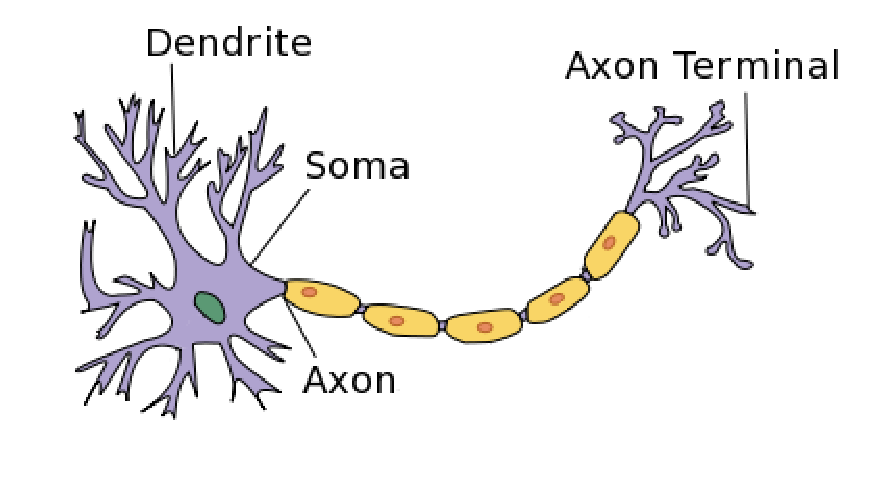
\includegraphics{neurone-diag}
}
\caption{Biological Neurone}
\label{fig:neurone:biological}
\end{figure}

Biological Neurones are cells in the nervous system and brain that process and transmit information through electro{}-chemical signals. They are the primary cell found in the brain and spinal cord of animals. There are many types of neurone and many of them interface with different aspects of a biological system, such as muscles or sensory receptors.

The basic neurone consists of a cell body called the {\textit{soma}} and a long thin {\textit{axon}}. The cell body has a dendritic tree which receives electro{}-chemical signals from other neurones. The axon has tree terminals which propagate the signal from the neurone to the next neurones. The signal is transmitted by the release of a neurotransmitter chemical into the {\textit{synaptic cleft}} (or just synapse) which is a gap between these terminals and the dendrites of the next neurone.

Communication between neurones is called synaptic transmission. This is triggered by action potential, the propagating electrical signal which is produced by the electrically excitable membrane in the neurone. Synapses connect the terminals to the dendrites of neurones; they are capable of either increasing or decreasing the membrance potential of neurones they are attached to.

The human brain has about $10^{11}$ neurones with each on average having 7,000 synaptic connections per neurone\cite{bioneurones}.
}

\subsection{Artificial Model of Neural Networks}
{
An Artificial Neural Network (ANN) is a computer{}-based model
representing a biological neural network. An ANN consists of a
collection of neurons, interconnected by synapses. A neuron is in
essence a mathematical function to model the output of a biological
neuron in the brain, given a set of inputs. Synapses have weights
(represented by ${\omega}$) that are used as inputs for the
neuron's mathematical function.
}

\subsection{Types of Neurons}
\subsubsection{Perceptrons}
{
The perceptron takes a vector of real input values (from the charge (\textit{x}) from its input synapses; let these be represented as \textit{c} = \textit{x}\textsubscript{1} * ${\omega}$\textsubscript{1} + \textit{x}\textsubscript{2} * ${\omega}$\textsubscript{2} + \textit{x}\textsubscript{3} * ${\omega}$\textsubscript{3} + {\dots} + \textit{x}\textsubscript{i} * ${\omega}$\textsubscript{i}) and outputs a value to each of its output synapses depending on a threshold function. There are a variety of threshold functions\cite{mitchell} that can be used to influence the perceptron's behaviour, for example;
}
\newpage
\begin{itemize}
\item {
The step function outputs 1 if \textit{c }exceeds the threshold, 0 otherwise.
}
\item {
The sign function outputs 1 if \textit{c} exceeds the threshold, {}-1 otherwise.
}

\item {
The linear function simply outputs \textit{c}.
}
\end{itemize}
\subsubsection{The Sigmoid Unit}
{
An extension to the perceptron model, the logistic sigmoid unit, instead operates over a differentiable continuous output function. The logistic sigmoid function calculates the output as  
$\mathit{output}\ =\ \frac{1}{1+e^{-c}}$

This tends towards 1 as {\textit{c}} increases, and towards 0 as {\textit{c}} decreases; it thus is not entirely dissimilar to the step function, except in that it is instead a continuous {\textit{squash}} function. Other squash functions are sometimes used, including those with some constant before the {\textit{c}} term in the logistic sigmoid function, or using the hyperbolic tangent function {\textit{tanh}}.
}

\subsection{Network Topology}
{
With the concept of the perceptron in place, the logical next step is to
connect them in an Artificial Neural Network. The most common way of
doing this with perceptrons is in a feed{}-forward layered graph. In
this topology, the network is laid out as a series of layers of any
number of perceptrons. Each layer is fully connected to the next (i.e.
each perceptron in layer \textit{i}\textup{ is connected to each
perceptron in layer }\textit{i+1}\textup{). There is thus a forward
flow of charge, from the inputs to the network through each layer until
the outputs are reached. The choice of number of perceptrons in each
layer is important in deciding the potential accuracy of the network as
a functional system.}
}
\begin{figure*}[t]
\centering
\scalebox{0.5}{
	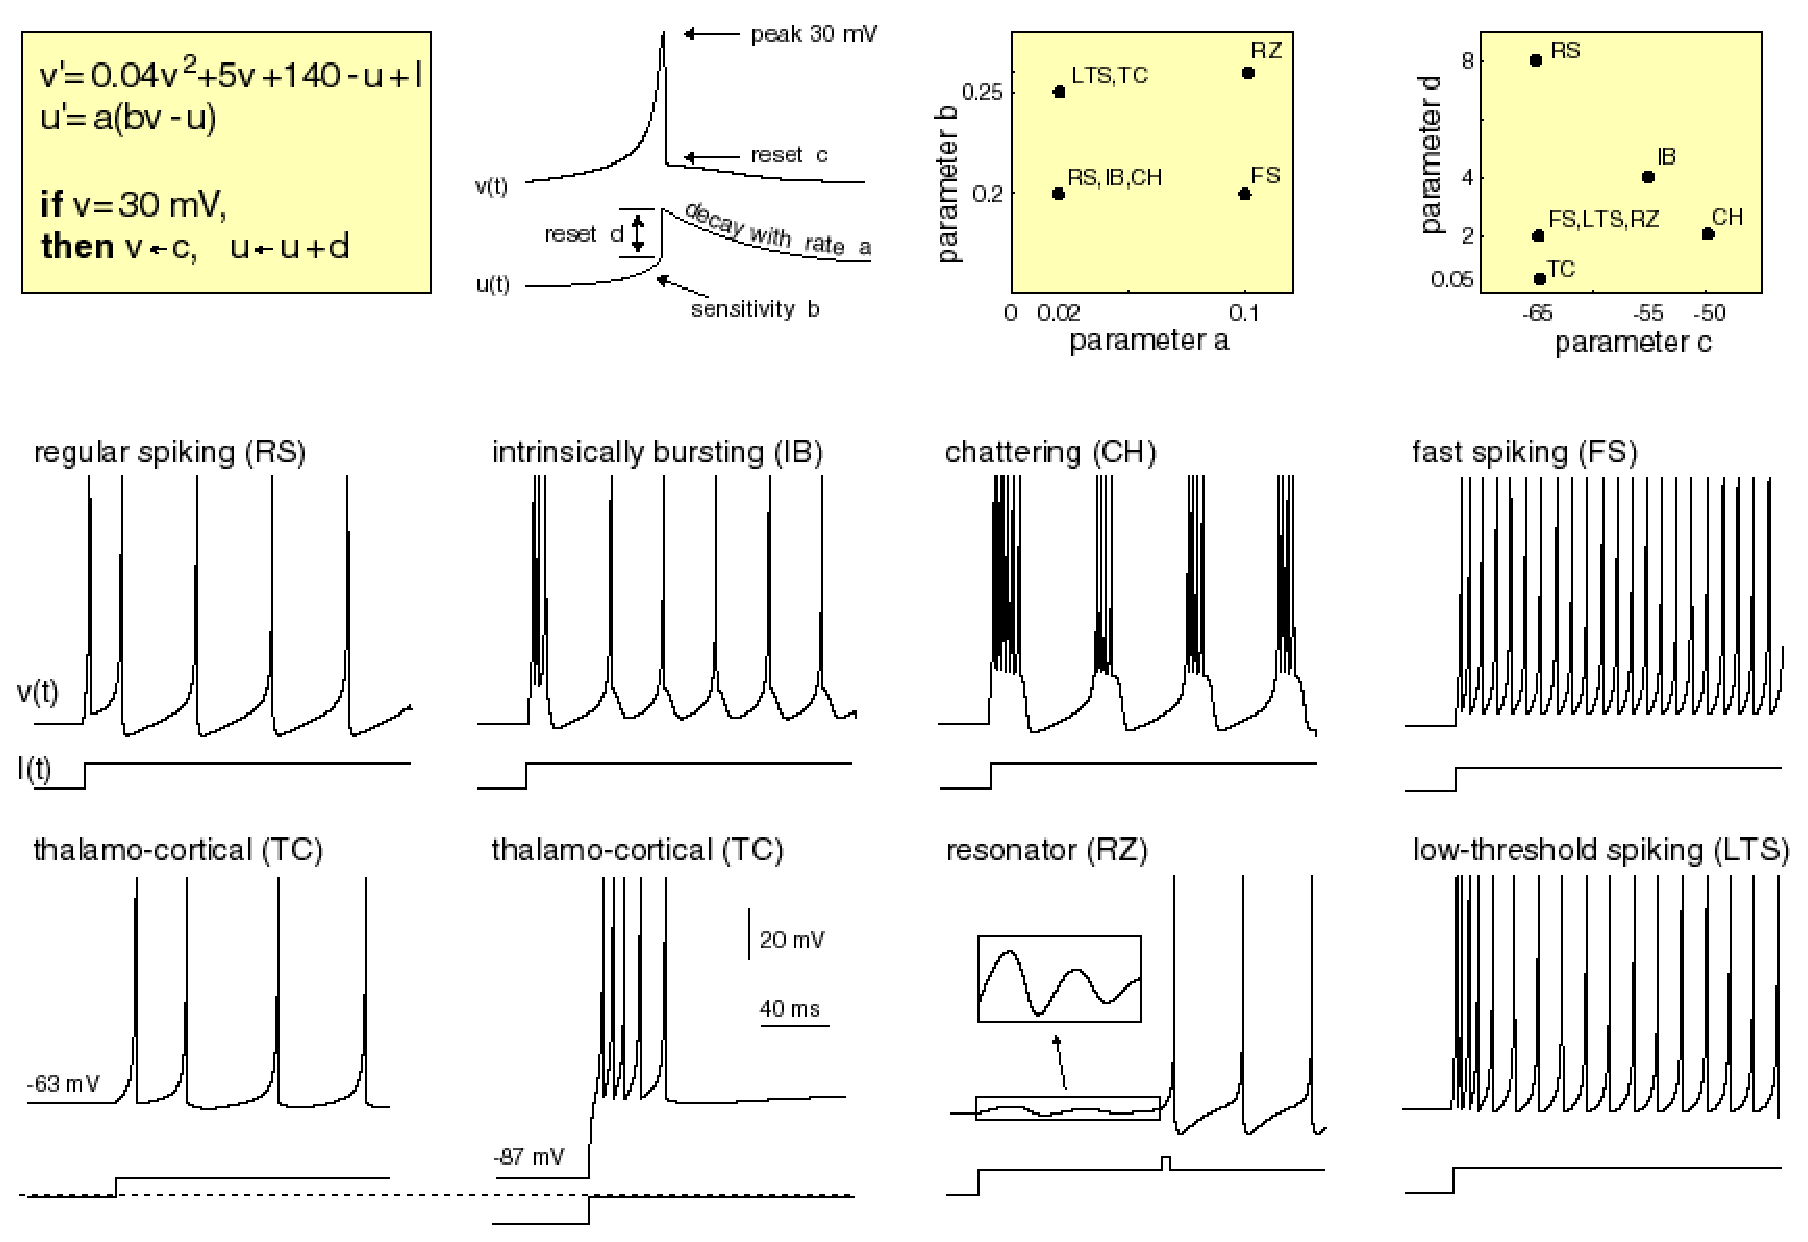
\includegraphics{spiking}
}
\caption{Spiking Neurone Behaviour}
\label{fig:anns:spiking}
\end{figure*}

\subsection{Training}
{
Training a network of perceptrons (be they sigmoid units or not)
requires the notion of a set of \textit{inputs}\textup{ and
}\textit{targets}\textup{ that the network must learn; as such, it is a
supervised learning paradigm. Within this, any number of algorithms may
be used to perform the actual training. Typically these algorithms run
for a given number of maximum iterations, or until some ``stop''
condition is met; e.g. a target accuracy.}
}
\subsubsection{Random Training}
{
Perhaps the simplest (and least efficient!) training methodology is the
random trainer; it simply modifies the synaptic weights at each level
of the network randomly and re{}-runs the inputs through the network.
If the accuracy of the network has improved as a result of the weight
changes, the changes are deemed a success and kept; otherwise they are
rolled back and the process repeated.
}
\subsubsection{Back Propagation}
{
The first step in back{}-propagation training is the ``feed forward''
step. In this, the inputs are run through the network and its outputs
are compared to the targets. The trainer then calculates an error value
for each output. The synaptic weight of each synapse between the output
layer and the one before it are used to determine how much each synapse
``contributed'' to this error, and thus by how much it should be
altered to compensate for the error. At this point the trainer requires
a notion of the ``learning rate''; the proportion of the error by which
to alter the synaptic weights. These factors are all combined to decide
the amount by which to alter the synaptic weights at this layer. Next
comes the back{}-propagation step; these weighted errors are propagated
back to the previous layer of the network as their ``target error'',
and the process repeats. This continues until the input layer is
reached.
}


\subsection{Advanced ANN Models}
\subsubsection{Spiking Neurons (Excitatory and Inhibitory)}
{
In reality, biological neurons are not nearly as simple as the
perceptron's model of them. Perceptrons fail to model
the temporal aspects of firing in the brain; neurones take time to
charge and then fire in spikes across their synapse. This also takes
time. Furthermore, they then have a period of reduced susceptibility to
charge {--} a so{}-called ``recovery period'' in which it requires a
very great amount of charge indeed to cause them to fire. Finally,
there are multiple types of neurones {--} those that excite other
neurons, and those that inhibit their firing.

Hodgkin and Huxley\cite{hodghux} first modelled these neurones mathematically, but their model was too complex to be able to scale and compute with. Eugene Izhikevich pioneered a simple model (Figure ref{fig:anns:spiking}\footnote{Electronic version of the figure and reproduction permissions are freely available at www.izhikevich.com}.) of spiking neurones\cite{izhikevich:simple} that was efficient enough to run large networks (\~{}1000 neurones) in real{}-time with millisecond precision. It almost exactly models the spike{}-timing dynamics of the observed firing patterns in a rat's cortex.
}
\subsubsection{Polychronization and STDP}
{
A later Izhikevich investigation\cite{izhikevich:polychron} showed that it was possible to compute using these spiking neurones, and to train the network in a very similar manner to how a biological brain learns. The fundamental principle of STDP, or Spike{}-Timing{}-Dependent Plasticity\cite{izhikevich:stdp}, is the Hebbian{}-based learning rule; to increase the strength of synapses between neruons that fire at approximately the same time. By the same token, synapses between neurons that fire at very different times are decreased in strength. In this way, the network forms a sort of spatial and temporal associative memory.

Suppose one were to present a spike of input at a cluster of neurons
{\textbf A} on a randomly initialised homogenous network. It may
cause a few other neurons it is connected to fire semi{}-randomly. If
one were then to present input spikes at two clusters simultaneously,
{\textbf A} {\textit {and}} {\textbf B}, and train the network with STDP
then it would learn that association. If a spike were presented at
either {\textbf A} or at {\textbf B} then the network would spike
automatically at the other.
}

\section{Architectural Design}
\subsection{Design Rationale}
{
As highlighted in our introduction, it is integrally important that the ANNE system is architected in such a manner as to be modular, pluggable, and highly configurable. To achieve this, the architecture of the system needed to be carefully selected at the start of the design process, and strict principles maintained throughout.

Two early decisions were taken to facilitate this. The first of these was to implement the primary components of the system as singleton {\textit{services}}, thus making it easy to reduce coupling and implementation specifics. Furthermore, we elected to split ANNE into three distinct components. The first of these would be the {\textbf{Framework}}; this provides basic programming constructs that would be useful for many applications, and is in no way specific to ANNE or to Neural Networks. On top of this was constructed a set of Neural network APIs, and a graphical user interface built atop the Eclipse SWT widget library. This forms the {\textbf{ANNE Environment}}. The final section of the project are a collection of {\textbf{Plugins}}, designed to extend the behaviour of the basic environment and facilitate complex and user{}-friendly interaction with the Neural Network.

\begin{figure}[t]
\centering
\scalebox{0.8}{
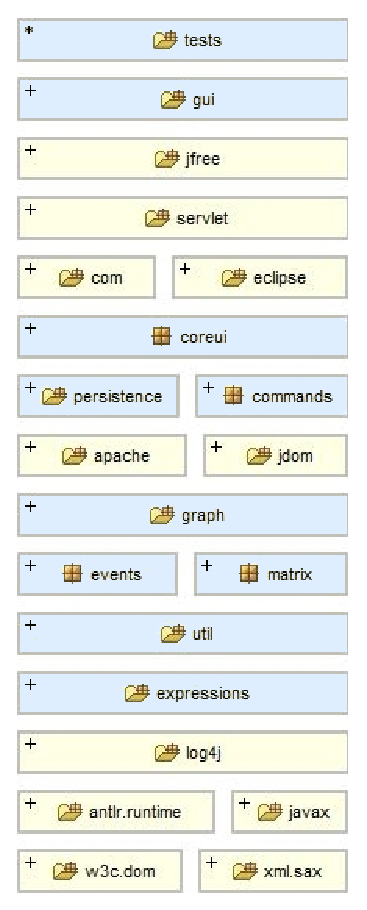
\includegraphics{externaldependencies}
}
\caption{Structure chart of internal (blue) and external (yellow) dependencies}
\label{fig:arch:external}
\end{figure}

The package structure of the project was designed to permit separation of these three concerns across their relevant sections. Plugins pertaining to the GUI, for example, belonged in a sub{}-package of {\textit{gui}}. Basic utility classes belonged in a {\textit{util}} package. Over{}-all, the namespace for the entire project was (according to standard Java naming convention), {\textit{uk.ac.ic.doc.neuralnets}}. With a correctly designed structure, it should be feasible to remove any package of interest, along with its dependencies, and to utilise it outside of the rest of the ANNE environment. Furthermore, it is integrally important that dependency leakage is avoided; no GUI{}-specific libraries or components may appear in the Neural Network packages, for example, so that the neural network may be run in a headless server environment, or as part of some alternative UI.

The final architecture's separation (and its full dependency layering) can be seen in Figure \ref{fig:arch:external}. As is clear from the lack of back{}-references, it is simple to (for example) replace the entire GUI package, built on SWT, with a CLI interface, or even one based on a client{}-server technology. This is made clearer with the package dependency hierarchy in Figure \ref{fig:arch:internal}.

\begin{figure}[t]
\centering
\scalebox{0.5}{
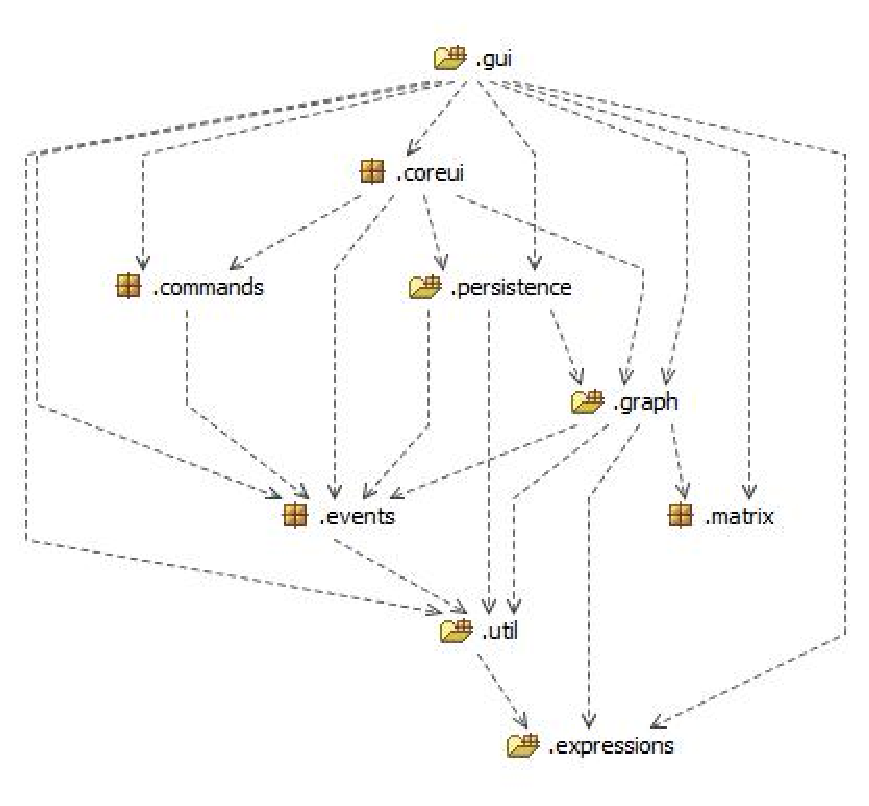
\includegraphics{projectdependencies}
}
\caption{Internal package dependencies}
\label{fig:arch:internal}
\end{figure} 
}
\subsection{Optimisation}
{
This final architecture is by no mans a ``perfect first draft". A large number of design iterations went into removing all back{}-references from the architecture and ensure packages were completely self{}-contained. One invaluable tool in performing this optimisation was the commercial Structure101\cite{structure101} (also responsible for the above diagrams). This excellent tool highlighted any back{}-references and tangles in our code, and facilitated the process of repairing our structure. Unfortunately, it is an expensive piece of software and could only be employed for a 15{}-day trial period; for this reason it was not used until the end of the project's life{}-cycle, in its final refactoring stage. At this point the architecture was approximately 50\% tangled, but had strong cohesion. By the time refactoring was complete, it exhibited no tangles at any package level. The only remaining tangles were of two or three classes, such as those which required (for efficiency of implementation and development) pointers to each other, such as in our directed graph implementation.

The most significant piece of this refactoring was in the GUI package. Most activity in the GUI was processed by a single facade class, the {\textit{GUIManager}}. To remove this absolute dependency from all UI classes that were not SWT specific, two interfaces were created in a new {\textit{coreui}} package, which abstracted out the behaviour of an ``Interface Manager", and one that was capable of Zooming into a Neural Network. By doing this, the Main class of the application could perform dependency injection of the {\textit{GUIManager}} into these classes.
}

\section{Framework}
\subsection{Introduction}
{
\begin{figure}[t]
\centering
\scalebox{0.5}{
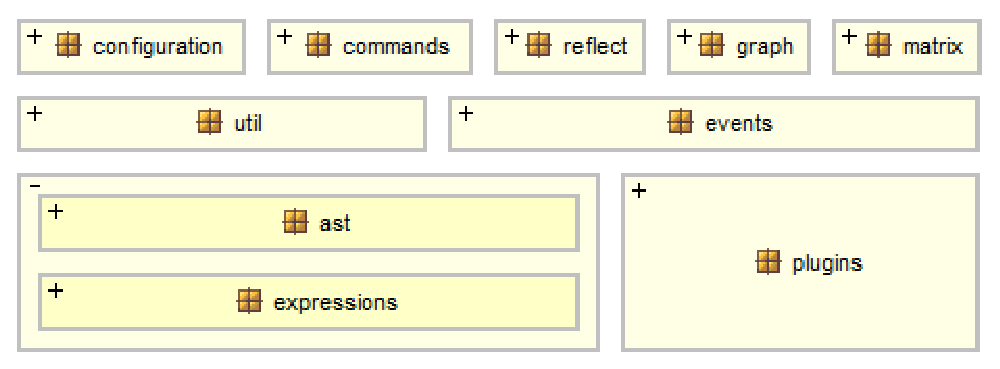
\includegraphics{Framework}
}
\caption{Framework Architecture}
\label{fig:framework:arch}
\end{figure}
As discussed previously, the framework of the system (Figure \ref{fig:framework:arch}) provides a basis of eight key services and interfaces upon which the rest of the system is built. These are completely generic and capable of providing their functionality to any type of application.
}
\subsection{Expressions}
{
The first of these services was for Expressions. These are provided as a set of tools for evaluating simple mathematical expressions, including support for dynamic variables and a variety of built-in functions (hyperbolic, trigonometric, exponential etc.)

There are two versions of this package available; the first supports a simple ``parse-and-evaluate" model, while the second version builds an abstract syntax tree and has better support for variables in expressions, as well as being more efficient. We will here focus on the AST Expression package.

\begin{figure}[t]
\centering
\scalebox{0.4}{
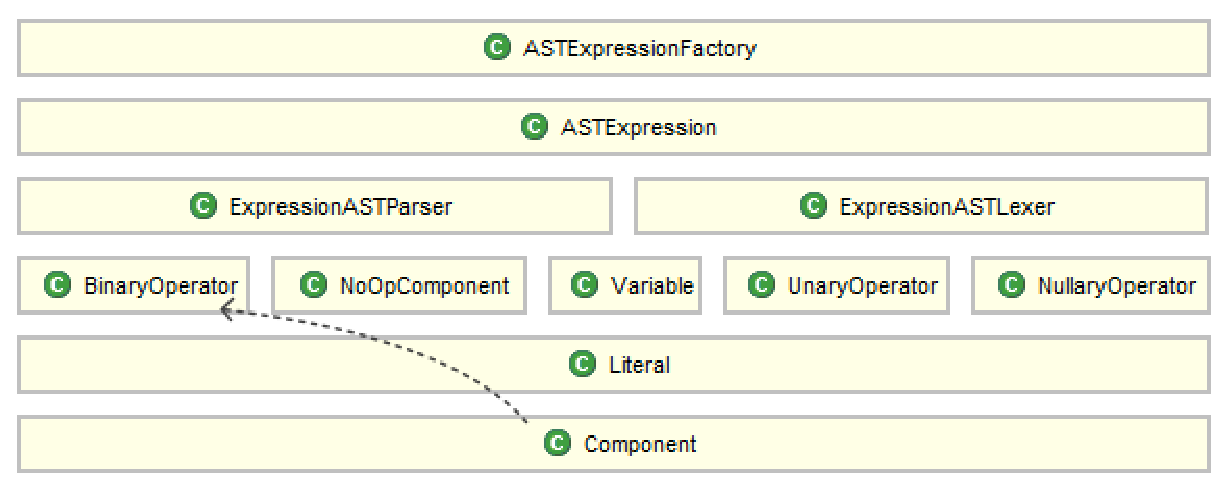
\includegraphics{ASTExpressions}
}
\caption{Framework: AST Expressions}
\label{fig:framework:ast}
\end{figure}
AST Expressions are built on top of the ANTLR parser generator. This is used to convert a grammar into the parser and lexer, seen in the middle of Figure \ref{fig:framework:ast}. Below this the abstract syntax tree can be seen; it is comprised of a tree of Component objects. These are either Literal values, or functions (be they nullary, unary, or binary). They are responsible for performing the operation assigned to them, as instructed in the parser. They also store pointers to their child nodes, and are capable of identifying any variables within themselves (recursively).

The abstract Component type has some knowledge of the types of expressions, and uses this to do simplification in bracketing according to the standard mathematical order of operations. While parsing occurs, the constructors of the operators all handle simplifaction of constant term expressions as far as possible.

The ASTExpression class wraps the behaviour of ANTLR and the syntax tree in a simple to use object. When using it, a developer simply passes in an expression to parse and it will instruct ANTLR to parse it. It can then bind variables based on the contents of an {\textit{@BindVariable}} annotation. This annotation permits a developer to annotate their code with the `getter' methods to bind variables, the name of the variable to bind to, and (optionally) whether the variable is dynamically bound (i.e. whether to re{}-bind its value in the tree every call, or just once).

Extensive profiling was conducted over the AST Expression classes to optimise their operation, as they are fundamental to the operation of the neurone classes, as we will see later. One of the primary causes of inefficiency was the Java reflection system for annotations; caching this data increased the speed of these by approximately 20\%. The efficiency was further improved by altering ASTExpressions to be created as Flyweight objects, cached in a {\textit{HashMap}} by the {\textit{ASTExpressionFactory}} service.
}
\subsection{Matrices}
{
\begin{figure}[t]
\centering
\scalebox{0.5}{
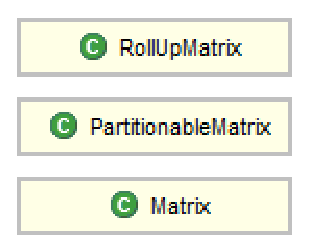
\includegraphics{Matrix}
}
\caption{Framework: Matrix Package}
\label{fig:framework:matrix}
\end{figure}
The Matrix package (Figure \ref{fig:framework:matrix}) offers three utility classes for dealing with vector or matrix data. The {\textit{PartitionableMatrix}} class extends this with the concept of {\textit{partitioning}} a matrix such that it `appears' to be only a sub{}-matrix of itself. Finally, the {\textit{RollUpMatrix}} is capable of `rolling up' to a particular size; that is, it transforms itself from a Matrix\textless T\textgreater{} to a Matrix\textless Matrix\textless T\textgreater{}\textgreater{} of smaller dimension, where the original matrix is split into a series of equivalent size sub-matrices in the new output.
}
\subsection{Plugin Management}
{
\begin{figure}[t]
\centering
\scalebox{0.5}{
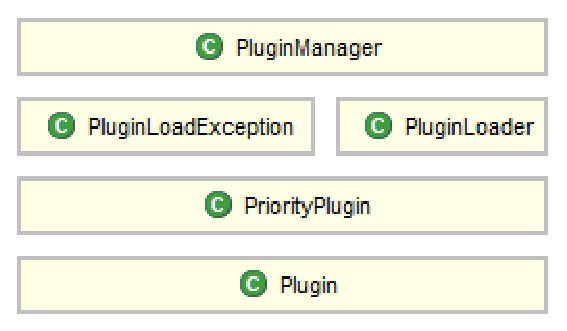
\includegraphics{Plugins}
}
\caption{Framework: Plugin Management}
\label{fig:framework:plugins}
\end{figure}
The plugin system (depicted in Figure \ref{fig:framework:plugins}) is the bedrock upon which the rest of ANNE is built. It forms the basis for all of its flexibility, modularity, and extensibility. As such it was integrally important that it was designed to be as effective as possible, whilst remaining easy to use {--} both in code and for the end{}-user of the system.

The guiding principles in the design of the plugin system were speed and ease of extension. It needed to be able to load plugins without a perceivable lag in responsiveness, and it needed to be easy for users to add more plugins once they have installed the system. In order to achieve this, it was decided that the file{}-system would be used to organise the plugins, according to Type and Plugin Name. Thus, we have a directory hierarchy of:

\texttt{
~~~ plugins/InterfaceType/PluginName.class
}

For example, a user might have:

\indent\texttt{~~~ plugins/SaveService/XML.class} \\
\indent\texttt{~~~ plugins/SaveService/Serialisation.class} \\
\indent\texttt{~~~ plugins/LoadService/XML.class} \\
\indent\texttt{~~~ plugins/LoadService/Serialisation.class} \\
\indent\texttt{~~~ plugins/Trainer/BackPropagation.class} \\
\indent\texttt{~~~ ... et cetera.}

In this way, adding a new plugin to be loaded is simply a matter of dropping it into the correct plugin directory. The plugin {\textit{.class}} file is simply a compiled Java class, as output by the {\textit{javac}} compiler. The plugin name need not be the same as its class name; this should be a more user{}-friendly name to describe its purpose.

From a developer's perspective, the {\textit{PluginManager}} offers two primary utilites. First, it is capable of listing all plugin names of a given type. This permits a developer to dynamically expand their code as the plugins are added. Secondly, it will instantiate an instance of a plugin for the developer based on Plugin Name, and its type. Using Java Generics it is feasible to do this in a type-safe manner, without the developer having to cast, increasing the safety and integrity of their code.

When a plugin is requested, the manager forwards the request to a custom ClassLoader, the {\textit{PluginLoader}}. This first checks its cache for that class. If it is not found, then the loader attempts to read it from disk, and use the standard Java ClassLoader methods for defining a class from a stream of bytes. It is possible that this may throw a LinkageError if that class has been previously defined; for example, if an objcet in memory has a reference to a plugin class directly, not through the plugin manager, then it is possible that the class is defined twice. In this case, the loader can simply fetch a Class of the source type from the JVM, cache it in its internal cache, and return it. The Plugin Manager then generates a new instance of this class, and uses the {\textit{Class.cast()}} method to cast from the returned Object to the requested type.

In general, profiling shows that the PluginManager is very efficient, and generally either hits its cache, or spends most of its time waiting for a Java native method to define the class. One area in which it could be improved is that of dependency management. It currently has no concept of the dependencies of a given plugin; if a plugin depends on other classes (or even contains inner classes), these {\textit{must}} be available on the class path. One could envisage an improvement to this that were capable of loading plugins with a manifest from a JAR file. Initially we avoided such an implementation in an effort to speed up the code (decompressing the JAR may slow down the implementation significantly), instead opting for a run{}-script to assemble dependencies from a {\texttt{plugins/lib}} directory.

One extension on the original design that was implemented through the project's life cycle is the notion of an abstract {\textit{PriorityPlugin}}. This includes a numerical ``Priority", and falls back to ordering based on the lexical form of the plugin name. The plugin implements the Java {\textit{Comparable}} interface, permitting the plugins to be placed directly into a {\textit{SortedSet}} and retrieved in their specified order. Nothing prevents a plugin developer from overriding this {\textit{compareTo}} method, should they require some alternative behaviour.
}
\subsection{Event Handling}
{
\begin{figure}[t]
\centering
\scalebox{0.4}{
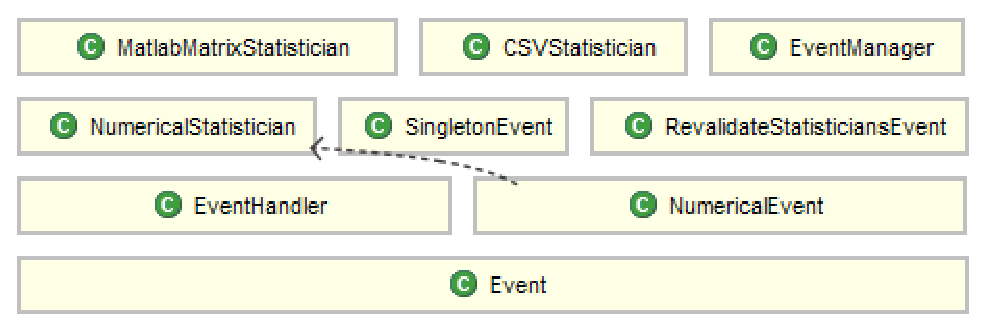
\includegraphics{Events}
}
\caption{Framework: Event Handling}
\label{fig:framework:events}
\end{figure}
The Event Handling subsystem (represented in Figure \ref{fig:framework:events}) provides a generic means for events to be fired, and to be handled by zero or more pluggable event handlers. Its design permits for a handler to by synchronous (``Do not return control to the firing method until this handler has finished executing") or asynchronous (``Execute this handler as soon as possible after the event is fired, but it is not totally time critical"). There need be no lmitation on how much (or, indeed, how little) data is stored in an event; the entire object should be simply passed into its registered handlers in turn to handle it.

The {\textit{EventManager}} is implemented as a singleton, containing two sets of mappings from Event Class to a List of {\textit{EventHandler}} objects; one representing the asynchronous handlers, and one for the synchronous. When an event is fired into the system, it is first added to an event Queue (in fact a {\textit{LinkedBlockingQueue}} for concurrency control) for processing by the asynchronous handlers. It is then passed into a {\textit{handle}} method, responsible for firing an event at each of its handlers from a given mapping. This same method is used by the asynchronous dispatcher thread, which {\textit{take()}}s an Event from the end of the queue before handing it off to the same {\textit{handle}} method.

When an event is handled, first its class is determined, and it is fired at all handlers registered for that Event class. If the super{}-class of that event class also happens to be an Event class, the handle method is recursed upon to fire the event at all handlers registered for the super{}-class, and so on until the given class is no longer a sub{}-class of Event. In this way, a more general Event type may be used in order to require a handler to be registered for multiple event types at once.

One example of this in use is a special Event type; the {\textit{RevalidateStatisticiansEvent}}. This is an abstract event class which has a handler registered by the {\textit{EventManager}} itself. This handler iterates over the collection of all handlers registered to the {\textit{EventManager}}, checking to see if they are valid. An {\textit{EventHandler}} may inform the {\textit{EventManager}} that it is no longer valid and thus cannot accept events. If this is the case, when a {\textit{RevalidateStatisticiansEvent}} is fired, the {\textit{EventManager}} may re{}-create these {\textit{EventHandlers}} using the {\textit{PluginManager}}.

A pair of convenience classes are provided; the {\textit{NumericalEvent}} interface, and the {\textit{NumericalStatistician}} abstract class. These permit a statistician to access so{}-called ``numerical" events as rows of data. This is the principle the CSV and MatlabMatrix statisticians operate over; the implementing event simply must provide one `row' of data for the statistician to process. It does this by having the {\textit{Event}} push its data through into the {\textit{NumericalStatistician}} as a var{}-args method call, thus making it easy for the event author to provide their data, and for the handler developer to process it. The default implementation simply stores a list of lists of Double values, for ease in later processing.

When profiled, it was determined that a large portion of the time spent in the {\textit{EventManager}} was spent awaiting locks over global resources; it tended to use {\textit{synchronized}} methods, or {\textit{synchronized()}} over the {\textit{EventManager}} object for concurrency control. After some reasoning, it was determined that these locks could be tightened to last for less time, and to be more specific. A significant performance boost was gained by moving these to be {\textit{synchronized()}} locks over the specific resources required (e.g. the {\textit{asyncHandlers}} map)
}
\newpage
\subsection{Configuration}
{
\begin{figure}[t]
\centering
\scalebox{0.5}{
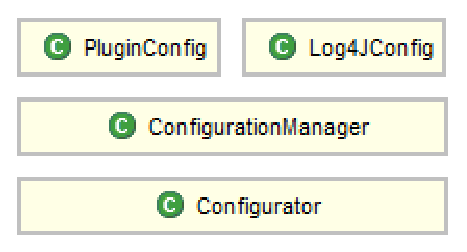
\includegraphics{Configuration}
}
\caption{Framework: Configuration System}
\label{fig:framework:conf}
\end{figure}
The next significant consumer of {\textit{Plugin}}s is the Configuration system (Figure \ref{fig:framework:conf}). This is designed to be a general{}-purpose means by which features of the software (including other plugins) can be configured at run{}-time. The primary {\textit{Configurator}}s in the system are to configure Log4J, the logging system, and the types of Neurone available. The format of configuration files are currently entirely up to the {\textit{Configurator}} developer; a future iteration of this design could perhaps provide more structure, and alleviate some of the strain of developing configuators by handling the parsing of the configuration file before the configurator is invoked.
}
\subsection{Commands}
{
\begin{figure}[t]
\centering
\scalebox{0.5}{
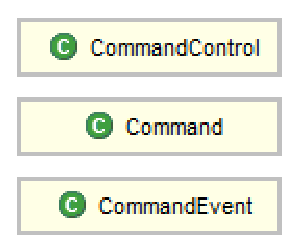
\includegraphics{Commands}
}
\caption{Framework: Commands Package}
\label{fig:framework:commands}
\end{figure}
The ability to undo mistakes is useful for all editor software, so early on in the project the decision was taken to include full undo and redo functionality. This feature is usually implemented in one of two ways: by recording internal state after each action then rolling back to a previous state when an action is undone (the Memento pattern), or by giving each action an undo method (Command pattern) that reverts all changes when called.

Saving and loading of network state already needed to be implemented in the persistence package, so it would be trivial to utilise this to record the current neural network after each action has been executed. However, large{}-scale neural networks can result in extremely large data structures and the time spent waiting for one to save after every action would make the program so slow as to be almost unusable. Creating an inverse method for each action requires more effort to develop, but the resulting performance is vastly improved.

Because of this, we implemented our undo and redo functionality using the Command design pattern (see Figure \ref{fig:framework:commands}). Each action that the user can execute and undo is encapsulated as a {\textit{Command}}, which is a {\textit{Runnable}} object containing {\textit{undo()}} and {\textit{execute()}} methods. These {\textit{Command}}s are managed by a central {\textit{CommandControl}} instance, which maintains stacks of {\textit{Command}}s that can be undone and redone as well as handling their execution to avoid deadlocks and concurrent edits.

This concurrency safety is handled by a dispatcher within the {\textit{CommandControl}}, which runs in its own thread and contains a multi-threading safe {\textit{BlockingQueue}} of commands to be executed. {\textit{Command}}s are added to this queue when they are created, undone or redone, and they are dispatched sequentially so no problems arise from simultaneous edits to a single data structure. An event is fired when execution of a command finishes so any interested components in the system can be informed of the changes. For example, the undo and redo buttons on a GUI's toolbar can check whether or not the undo and redo stacks are empty and enable or disable themselves accordingly.

Although each action is a separate command, many of them share functionality. For example, the {\textit{execute()}} method of a command to delete items, and the {\textit{undo()}} methods of a command to add items are functionally equivalent to each other. This behaviour can (and in general has in our implementation) been factored out into a single operation class, and is available to be used in any future actions that may require it.
}
\subsection{Graphs}
{
\begin{figure}[t]
\centering
\scalebox{0.5}{
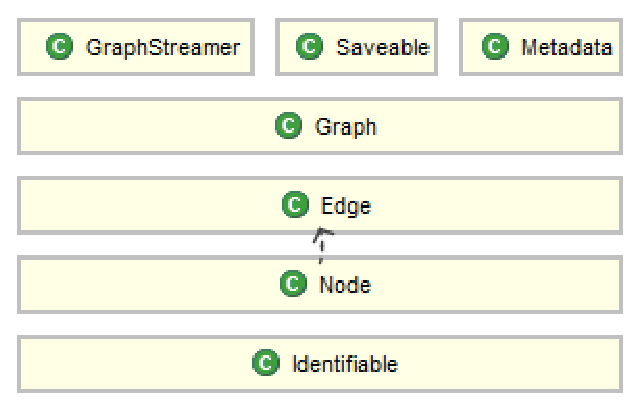
\includegraphics{Graph}
}
\caption{Framework: Graph Package}
\label{fig:framework:graph}
\end{figure}
As a modelling tool for Artificial Neural Networks, it was deemed important that ANNE was built upon a solid, but not overly complex, Graph implementation (Figure \ref{fig:framework:graph}). This implementation is essentially a directed {\textit{Graph}}, consisting of {\textit{Node}}s and {\textit{Edge}}s. The interface for {\textit{Node}} is generically parameterised with its {\textit{Edge}} type, and vice{}-versa; the {\textit{Edge}} is parameterised with the types of the {\textit{Node}}s at either end.

It was decided, for ease of use, that {\textit{Node}}s and their {\textit{Edge}}s should maintain back{}-pointers to each other, so that it was possible to navigate the graph from {\textit{Node}} to {\textit{Edge}} to {\textit{Node}}.

All elements in the {\textit{Graph}} implement the {\textit{Identifiable}} interface, which provides convenience methods for accessing and processing their universally unique identifiers. These permit any implementing code to refer to graph components by a persistent ID, rather than simply by memory pointer; of particular utility in, for example, statistical systems.

The {\textit{GraphStreamer}} class provides a convenient way for a developer to provide a {\textit{Graph}} and two transformer classes from {\textit{Node}} to a type of their choosing, and {\textit{Edge}} to another type of their choosing. These can then be used to stream the contents of the {\textit{Graph}} through to another type, in order to support simple type transformations (in a similar vein to a functional{}-programming `{\textit{map}}' function).

The final portion of the {\textit{Graph}} implementation of note is the Metadata system. This provides a simple but effective way of storing any information that is not directly a component of the {\textit{Graph}}, or its {\textit{Nodes}}, but that is still relevant. It stores its data as a collection of simple String \textless key, value\textgreater{} pairs.
}
\subsection{Reflection}
{
The final framework package we will cover is a set of Reflection helper methods. It was deemed important that the software solution's persistence system (to be discussed in detail later) was capable of retrieving and setting fields in an object in a uniform manner. One side effect of this work was to make it possible for a developer to retrieve and set values on a private Field, using Sun's {\textit{ReflectionFactory}}. Once this was done, it was possible to retrieve a Field object by reflection for the given class, and to mutate its internal private {\textit{FieldAccessor}} (responsible for reflecting into the field and getting / setting values) to instead operate over a method. This essentially provides JavaBeans{}-esque functionality to the Java programmer, permitting them to consider Methods and Fields as one collection of ``data".

To accomplish this, a few assumptions need be made. The {\textit{MethodPseudoAccessor}}, responsible for permitting a {\textit{Field}} object to back{}-end its logic to a {\textit{Method}}, attempts to seek setters and getters following the standard pattern of field ``someField" having mutators ``setSomeField(value)" and getter ``getSomeField()". The type of ``value" in the previous may be any of {\textit{Double}}, {\textit{Integer}}, {\textit{String}}, or {\textit{ASTExpression}} in our implementation. It is, however, feasible to extend this to support more types.

The absolute requirement for this system to function over {\textit{Field}} was, in fact, rescinded during development as an XML persistence library the project depended on ceased to be available. This library would only operate over arrays of Java {\textit{Field}}s. However, the package's utility was deemed to be sufficiently great that it was kept. In a future iteration of the software, a cleaner and more portable solution to this problem would be to define a ``Datum" type, which can back{}-end its getting and setting of values to either a {\textit{Field}}, or a {\textit{Method}}.
}

\section{Neural Networks}
\subsection{Overview}
{
With the solid foundations of the framework in place it was possible to create a fully{}-featured neural network model for our system. The model was required to emulate Izhikevich's spiking neurone networks as well as classic feed{}-forward artificial neural networks, both in their contstruction and execution. As the model would have to scale to contain millions of total components an efficient design was required to minimise resource usage and maintain responsiveness for the user. It was also required that neurone parameters be fully configurable during general use of the application.

A correspondence between Izhikevich's network model, specified in Matlab, and our own model needed to be created. Izhikevich's model relies on a number of matrices to hold data describing the neurone charges, synaptic weights and synaptic delays, as well as vectors to describe other neurone parameters. Since Java was being used it seemed apparent to model network components as discrete objects rather than using two-dimensional arrays in a more direct `port'. This design also enhanced the customisation and specialisation options for neurone parameters on a per neurone basis rather than requiring constant values for all neurones in a network. 

Neural networks are executed, or run, by performing discrete {\textbf{tick}} operations on them repeatedly. The ticks are propagated down from the root network to all components. For example, in a feed-forward network a single tick involves propagating charge from the input neurones, through the hidden layers, to the output neurones. In the spiking model a tick involves adding a random thalamic input to all neurones, calculating which neurones have fired and moving charge along the synapse from one neurone to another. This thalamic input is intended to model the activity of the thalamus in the brain; the portion of the brain devoted to processing external stimuli. Its random nature in Izhikevich's model is simply to cause network activity. When attempting to compute using these networks, large{}-scale random input is obviously not desirable.
}
\subsection{Design}
{
\begin{figure}[t]
\centering
\scalebox{0.5}{
	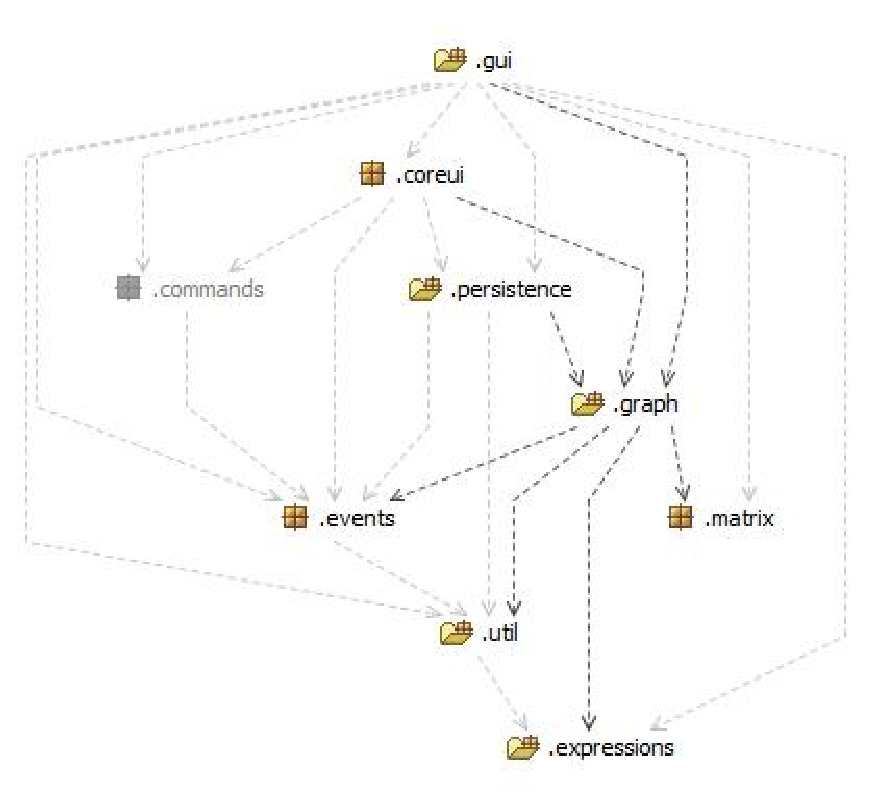
\includegraphics{GraphDependencies}
}
\caption{Dependencies on the Graph / Neural Network package}
\label{fig:neural:dependencies}
\end{figure}
\begin{figure}[t]
\centering
\scalebox{0.4} {
	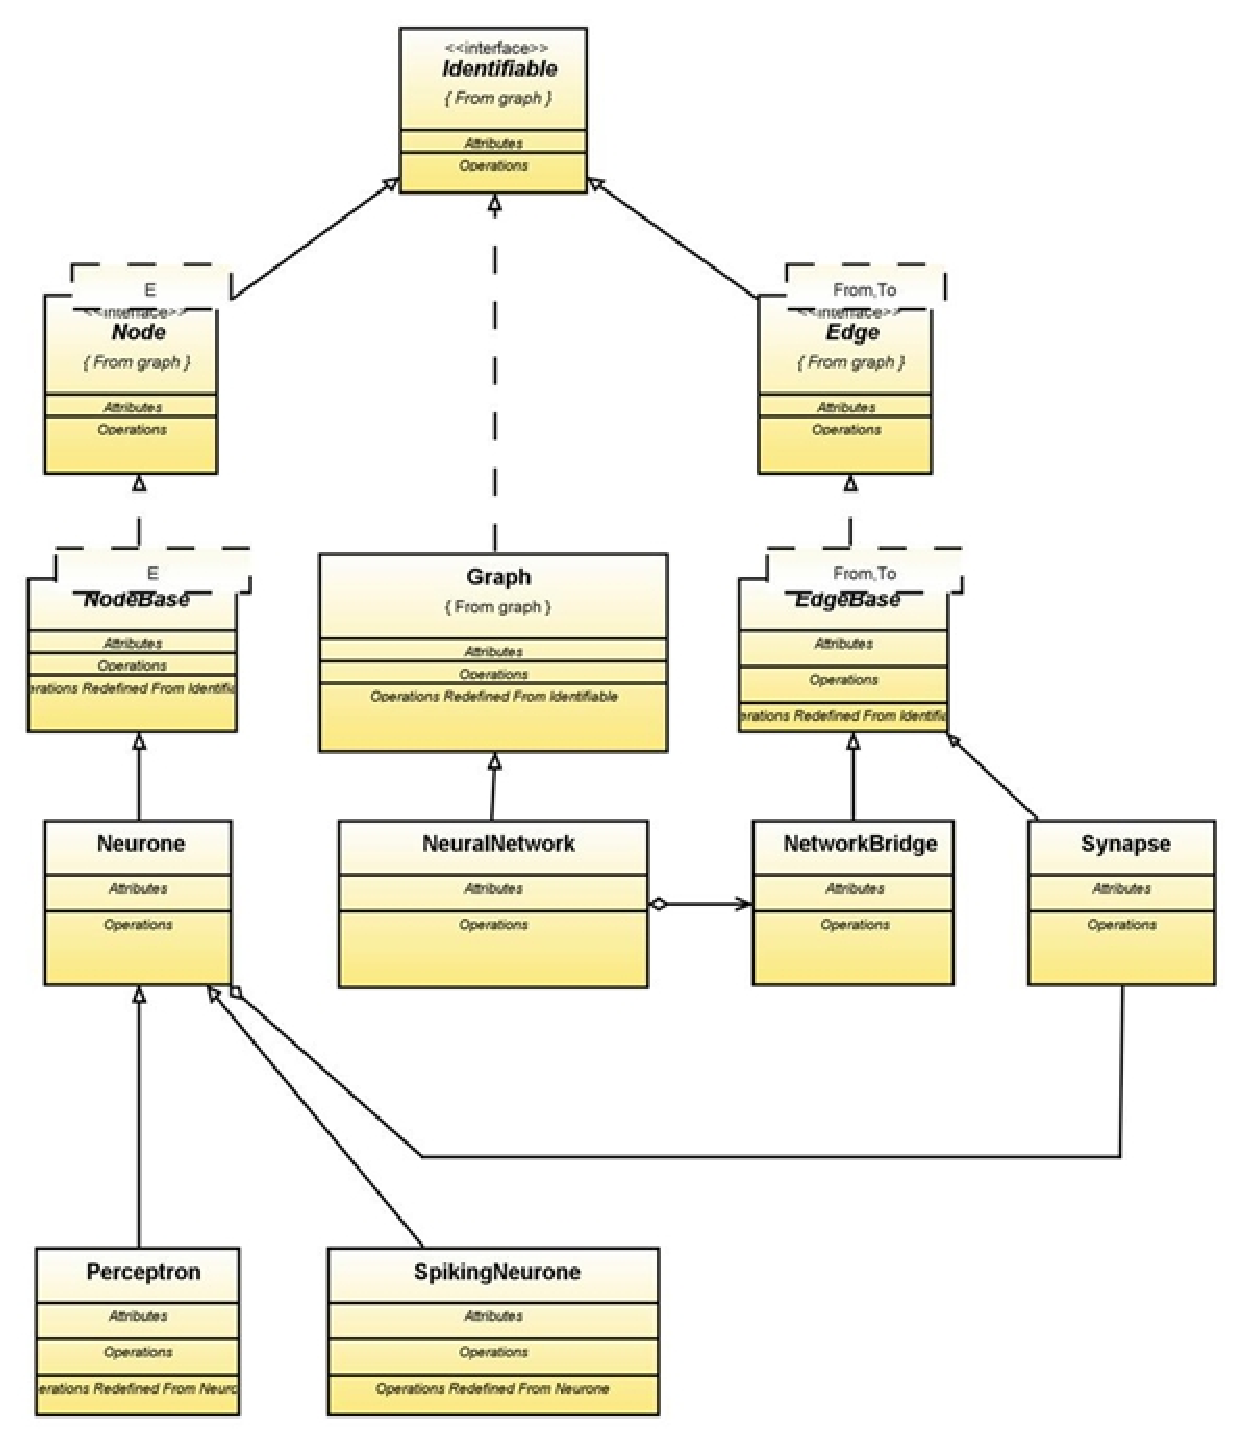
\includegraphics{NeuralUML}
}
\caption{UML Class Diagram of Neural Network Implementation}
\label{fig:neural:uml}
\end{figure}
There are four classes central to the model: {\textit{Neurone}} and {\textit{Synapse}}, {\textit{NeuralNetwork}}, and {\textit{NetworkBridge}}. Their implementations are specialisations of the general Graph service in the Framework. 

The lowest-level building block of a network is the {\textit{Neurone}}. {\textit{Neurone}}s are implementations of the {\textit{Node}} interface from the Graph framework, through a basic implementation of the abstract {\textit{NodeBase}} class. While {\textit{NodeBase}} controls aspects concerning abstract node connectivity in a network, {\textit{Neurone}} specifies the parameterisation such as squash function, trigger values and tick behaviour. 

The {\textit{Neurone}}s are connected together with {\textit{Synapse}} objects to form the basic network structure. {\textit{Synapse}}s extend {\textit{EdgeBase}}, which provides a fundamental abstract implementation of {\textit{Edge}}, simply adding synaptic weights.

{\textit{NeuralNetwork}} is a specialisation of the {\textit{Graph}} framework class. It polymorphically implements the {\textit{Node}} interface so that a {\textit{NeuralNetwork}} can contain both {\textit{Neurone}}s and other {\textit{NeuralNetwork}} nodes, allowing for self-containment similar to the directory structure on a file-system. {\textit{NeuralNetwork}}s also have the ability to tick, which is propagated to all {\textit{Neurone}}s and sub{}-networks contained within it.

{\textit{NetworkBridge}}s are {\textit{Edge}}s that connect together {\textit{NeuralNetwork}}s. They contain a bundle of {\textit{Edge}}s that connect {\textit{Node}}s inside the networks linked by the bridge. {\textit{NetworkBridge}}s are created implicitly when a node from one network is connected to a node from another network. For example, if {\textit{Neurone}} {\textbf{A}} in {\textit{NeuralNetwork}} {\textbf{X}} is connected to {\textit{Neurone}} {\textbf{B}} in {\textit{NeuralNetwork}} {\textbf{Y}} with a {\textit{Synapse}} {\textit{S}} then {\textbf{X}} and {\textbf{Y}} are first connected with a {\textit{NetworkBridge}} {\textbf{R}}, which contains {\textit{S}}.
\newpage

There are two further specialisations of {\textit{Neurone}}: {\textit{Perceptron}}, which is for use in feed-forward networks, and {\textit{SpikingNeurone}} which is the base class for use in spiking networks, and adds the parameters expected by Izhikevich's model.

Neurone parameters can be configured both while the application is running and offline. While the application is offline modifications can be made in the plain text file {\textit{nodetypes.cfg}} in the {\textit{conf}} directory. During program use the {\textit{Neurone Designer}} can be used; changes made in the designer can be propagated automatically to {\textit{nodetypes.cfg}}, using the Event System. This also makes it feasible to ensure UI components are informed of changes in a neurone type's parameters.

The creation of neural network components is controlled by specifications and factories in the {\textit{manipulation}} package. {\textit{Neurone}}s are created by the {\textit{NodeFactory}} using {\textit{NodeSpecification}}s. The {\textit{nodetypes.cfg}} file is parsed at application launch time by the {\textit{NeuroneTypeConfig}} configurator which loads the neurone parameter sets into the {\textit{NeuroneTypes}} registry. A {\textit{NodeSpecification}} can be requested from the {\textit{NeuroneTypes}} registry for a named neurone configuration. This {\textit{NodeSpecification}} can subsequently be passed to the {\textit{NodeFactory}} to create a concrete node instance. {\textit{NodeSpecification}} is extended by {\textit{SpikingNodeSpecification}}, {\textit{InhibitorySpecification}} and {\textit{PerceptronSpecification}} which provide default values for these implementations. 

{\textit{NodeSpecification}}s make extensive use of the ASTExpressions service of the Framework. This allows arbitrarily complicated mathematical expressions to be used for neurone parameters where necessary.

{\textit{Edge}}s are created by passing an {\textit{EdgeSpecification}} to the {\textit{EdgeFactory}}.

{\textit{NeuralNetwork}}s are created in a similar fashion, using {\textit{GraphSpecification}} types and the {\textit{GraphFactory}}. A {\textit{HomogeneousNetworkSpecification}}, a concrete {\textit{GraphSpecification}}, is created with one or more {\textit{NodeSpecification}}s and associated node counts as well as an edge probability. The edge probability defines the probability that a given node will be connected to another during network creation. This specification is passed to the {\textit{GraphFactory}} which is responsible for calling the {\textit{NodeFactory}} to create the various types of neurone objects, interconnecting the neurones with edges, and returning the resultant objects encapsulated in a {\textit{NeuralNetwork}} object. It is also possible to invoke the {\textit{GraphFactory}} with a custom transformer, which will select how to connect neurones together.

Also in the {\textit{manipulation}} package are the {\textit{InteractionUtils}}. These are a collection of miscellaneous convenience tools for interacting with {\textit{NeuralNetwork}}s in various important ways. There are utilities for finding the network that directly contains a given node, finding if a given network {\textbf{A}} contains a given network {\textbf{B}} and finding the lowest common ancestor of two nodes, i.e. the first network that contains both nodes. There are also tools for network birfurcation, connecting two nodes or two sets of nodes in a network, automatically creating the any required {\textit{NetworkBridge}}s, either fully or in a one to one manner. A control thread for concurrent running, stopping and resetting of the network is also contained in the {\textit{InteractionUtils}}.
}
\subsection{Input and Output Nodes}
{
The I/O Node system provides a simple and extensible way for running data external to the application through a neural network. For example, an {\textit{InputNode}} could be created to hash images into data arrays which could then be fed through a network. In a similar way, an {\textit{OutputNode}} could be created to convert network output to database identifiers and retrieve a database record pertaining to the recognised image; e.g. for application with a facial recognition network.

{\textit{InputNode}}s provide a matrix of data that is run through the network row by row. They can also provide a matrix of targets that can be used during training, each row of the target matrix corresponding to a row of the data matrix. {\textit{InputNode}}s are {\textit{Foldable}} (another interface) denoting that they support the notion of N-Fold testing. N-Fold testing divides the training data into two subsets: one that will be used for training and one for testing. After one fold of training and testing new subsets are created. This process is repeated until each item is used for testing. For example, for a data set of 100 rows, 1-90 are used to train and 91-100 to test, then 1-10 and 21-100 to train and 11-20 to test, and so on until all 100 rows have been used. This folding is implemented using the {\textit{PartitionableMatrix}} from the Framework.

{\textit{OutputNode}}s create a specified number of nodes which call an abstract {\textit{fire}} method when they fire, passing their index and charge. This gives the concrete node implementation full control over the data flowing out of the output nodes. A call to the abstract {\textit{setNodes}} method allows an {\textit{OutputNode}} to configure its internal systems when created.

Both the {\textit{InputNode}}s and {\textit{OutputNode}}s provide {\textit{recreate}} and {\textit{destroy}} housekeeping methods. The {\textit{recreate}} method may be invoked when configuration data is already in memory and the user need not be prompted for it again. {\textit{Destroy}} is a tear-down method, called when the node is removed from the display. 

When I/O Nodes are added to a network they must be connected up using the standard User Interface tools to do so; {\textit{InputNode}}s and {\textit{OutputNode}}s are both extensions of {\textit{NeuralNetwork}}, so can be manipulated within the network in exactly the same way.
}
\subsection{Training}
{
The training of neural networks is handled by pluggable {\textit{Trainers}}. The basic interface defines methods for setting the {\textit{InputNodes}} for the training data, the number of network ticks for a single test, a {\textit{trainOnce}} method that performs a single test run, and a {\textit{trainFully}} which trains to a specified accuracy / maximum iteration count.

One basic abstract implementation of the {\textit{Trainer}} is the {\textit{StepwiseTrainer}} which allows for housekeeping, such as synaptic weight adjustment, to be performed between each training iteration. The back-propagation trainer, random trainer and the granular random trainer all extend the StepwiseTrainer. The STDP (Spike{}-Timing{}-Dependent Plasticity) trainer implements the {\textit{Trainer}} interface itself.
}
\subsection{Events}
{
The neural network package uses the {\textit{EventHandler}} extensively so that other system modules can be notified of network events. During network creation, {\textit{NodeCreatedEvent}}s and {\textit{EdgeCreatedEvent}}s are fired when nodes and edges are created respectively, to provide progress information to the UI. When a network starts or stops running a {\textit{NeuralNetworkSimulationEvent}} is fired and {\textit{NeuralNetworkTickEvent}}s are fired each tick. Every time a node fires, a {\textit{NodeFired}} event is triggered and {\textit{NodeChargeUpdateEvent}}s are fired when nodes are charged. {\textit{NewNeuroneTypeEvent}}s are fired when the Neurone Designer creates a new neurone type. 
}

\section{Persistence}
\subsection{Overview}
{
\begin{figure}[t]
\centering
\scalebox{0.5}{
	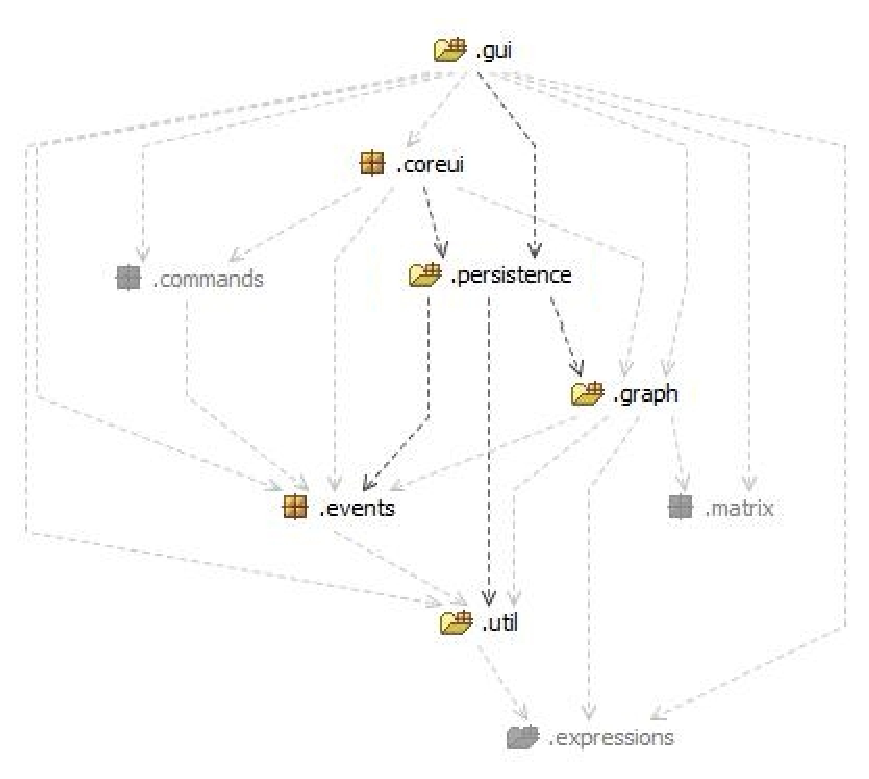
\includegraphics{persistencedepends}
}
\caption{Persistence's location within the framework.}
\label{fig:persistence:depends}
\end{figure}
Figure \ref{fig:persistence:depends} provides a view of how persistence rests within the application
framework in terms of its dependencies and the modules that depend on it. For obvious reasons, the user interface is dependent on the persistence module being present for the ability to save or load neural networks which have been
designed within the application. persistence depends on the model of
these networks, a few core utilities and events for serialization and
de{}-serialization of networks. This is coherent with the low coupled
design of the framework.

\begin{figure*}[t]
\centering
\scalebox{0.35}{
	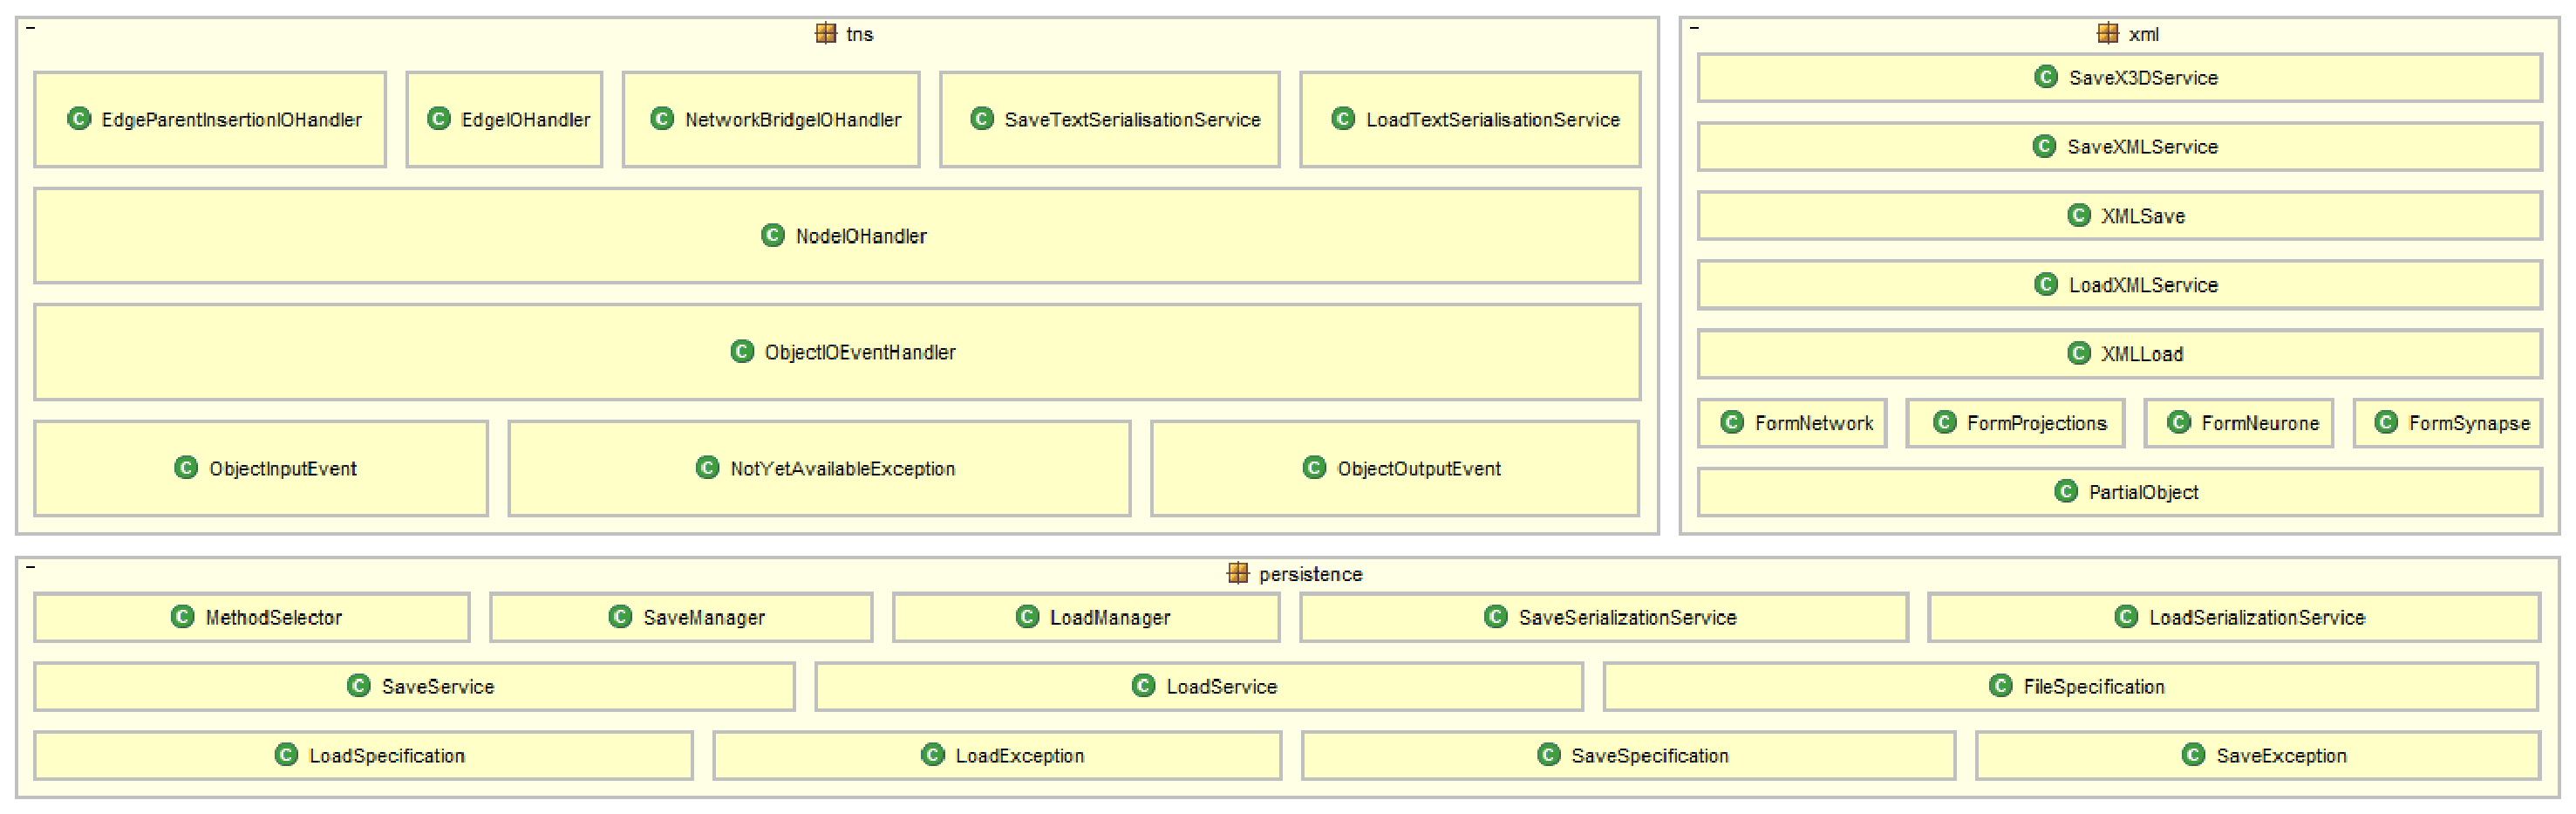
\includegraphics{PersistenceHierarchy}
}
\caption{Persistence Modules Implementation.}
\label{fig:persistence:hierarchy}
\end{figure*}
Figure \ref{fig:persistence:hierarchy} is an overview of all the classes and interfaces within the persistence module and their package separation. XML and TNS have their own packages as they require specific classes for their implementation, whereas the Java Serialization services make use of the Java's in{}-built ability to serialize objects to a persistable storage location. X3D is dependent on the XML system but required no other external classes apart from the base service for its persistence.
}

\subsection{Design}
{
The persistence layer has been designed, like many aspects of the
application to be completely modular and pluggable with new services. Furthermore its architecture is such that it is not, in its abstract form, directly related to saving and loading of neural networks. Instead it simply relies on the concepts of a "Saveable" object, "Persistable" data, and "Specifications" of saving, leaving the implementation details entirely up to the particular service. Adding a plug{}-in requires no existing code to be changed and the new plug{}-in to extend the {\textit SaveService} for saving networks, or {\textit LoadService} for loading networks. These abstract classes provide the method headers for creating persistence services. A new plug{}-in doesn't have to implement both loading and saving, as is the case with the X3D service which is only available for exporting networks.
\begin{figure}[t]
\centering
\scalebox{0.4}{
	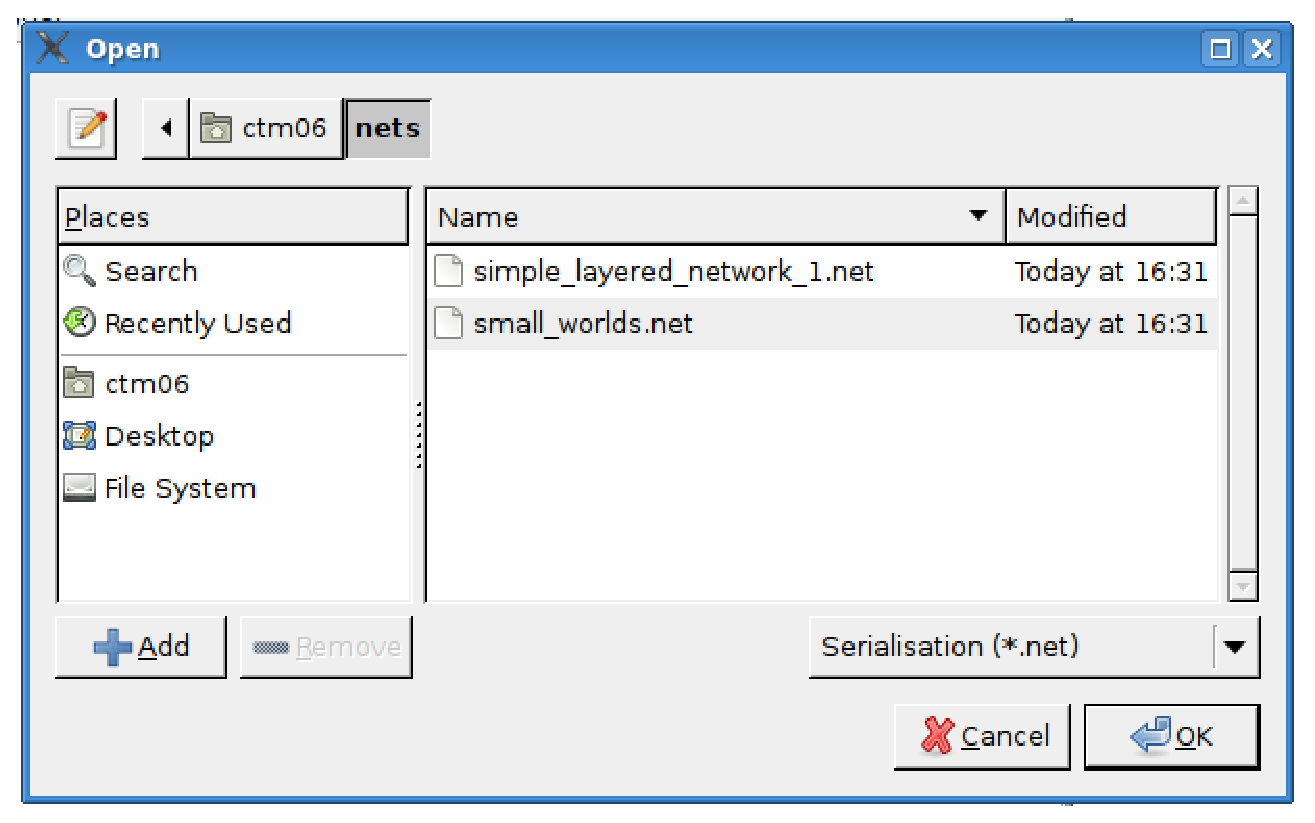
\includegraphics{opendialog}
}
\caption{View of Open Dialog}
\label{fig:persistence:open}
\end{figure}
A number of persistence plug{}-ins are provided with the standard
distribution, they are:

\begin{itemize}
\item { {\textit{Java Serialization\cite{java:ser}}} {--} The network is serialized using the Java Serializable and ObjectOutputStream interfaces; this is used as the default persistence option and preferred over the other modules, especially when not transporting the neural network to another application. This is because it is extremely fast and
guarantees that all information is persisted and will be loaded again. As the serialized network consists of the actual in-memory objects of our implementation, the only applications that would be able to make use of this format are those which use our framework for network representation. Files are given the {\textit{.net}} extension.
}
\item {{\textit{NeuroML\cite{neuroml}}} {--} This is the main persistence module for exporting to a number of other applications that also support the standard
NeuroML Layer 3 Network Schema for representing in neural networks. Import is also supported for taking NeuroML from other applications that also use this schema, allowing for some cross{}-application portability. The XML that is generated has been verified to be well{}-formed and NeuroML validated, meaning that other applications should accept this format without errors. Files are given the {\textit{.xml}} extension.
}
\item {{\textit{TextNetworkSerializer}} {--} A simple fact{}-based export
and import specification which outputs records of all the objects into
a plain-text format for storage. Like Java Serialization, however, it is a non{}-standard format which is only implemented by our framework so cannot be used for exporting to or importing from other tools. It does however have a low storage overhead compared to XML and performs faster than the Java Serializer. Files are given the {\textit{.tns}} extension.
}
\item {{\textit{X3D}} {--} A royalty{}-free open standards file format and run{}-time architecture to represent and communicate 3D scenes and objects using XML\cite{web3d}. We implemented only an export feature to X3D as applications that implement this standard are designed for viewing as opposed to modelling items. Furthermore the feature is implemented by an XSL transformation from our NeuroML that is generated and we chose not to implement an XSLT for transforming from X3D to NeuroML. Files are given the {\textit{.x3d}} extension.
}
\end{itemize}

Further plug{}-ins for persistence to expand the project's portability could include PyNN\cite{pynn} and the Neural Network Tool within Matlab\cite{nntool}.
}

\subsection{Implementation}
{
As previously mentioned, loading and saving functionality is abstracted out as far as possible into plug{}-ins; all loading and saving is handled by the Save and Load Managers, which is the last point in the core system before the request is passed to the plug{}-in. It is the Manager's job to take a load or save specification which includes information about where to write or read the data and also which plug{}-in to use to perform the persistence operation. The manager then loads the required plug{}-in before making the appropriate method
calls. The details of the specification are read by the plug{}-in and acted on accordingly.

Networks must be Saveable (and Serializable for Java Serialization) to be used with the {\itshape SaveManager} and save plug{}-ins, further still any object
that has parameters or variables that require persistance to storage must have them annotated with the annotation {\itshape @Persistable}. This is so that when an object is being persisted reflection can be used to retrieve all information from the object that needs to be exported. It is also used when loading persisted information and populating information in objects upon reading a persisted network back into memory.
}
\subsubsection{Serialization}
{
Serialization was the simplest implementation as it makes use of
Java's ability to serialize objects to file and allow
them to be read back in, as the loading plug{}-ins are used for when a
user wishes to insert a network from file into one which they are
editing currently. After the network is loaded, objects must have their
Ids regenerated to prevent Id conflictions.
}
\subsubsection{NeuroML}
{
NeuroML is implemented to conform to the NeuroML DTD, which specifies that networks and their neurons must be output followed by the synapses. This requires the NeuroML save service to buffer some information so that it can be output at the correct time. NeuroML does a breadth{}-first search of the network to discover all the networks and network bridges that are in the network being persisted.

Importing NeuroML is more interesting. Information is not only stored in a single tag, but multiple tags, including meta{}-data tags. This requires more information to be stored and lead to the {\itshape PartialObject} concept, which stores information temporarily, until the load is completed, and then will produce the concrete object with the stored parameters. More information needed to be stored because the XML parser that was used to read the XML was SAX (Simple API for XML)\cite{sax}. SAX is event driven and its output is dependent on what the parser's state; i.e. what it has read at a given time influences what you receive. The parser then acts depending on the type of tag seen; if it is an opening tag for a neurone, network or synapse then a partial object is placed on a stack. As further meta{}-data that is relevant to the last seen partial object  is encountered, it is added to the partial object on top of the stack. On closing tags for neurone, network or synapse, the partial object creates the complete object based on the parameters that it has stored and returns it. At the end of the document the network is connected up with sub{}-networks and the final network can be retrieved. Objects that require methods to be called other than the standard constructor when being loaded from persistant storage may do this by creating methods that are persistable but have no actual value, so that they are called as a kind of `pseudo-setter' when loaded; any further method calls and operations can be placed within that single public method.
} 
\subsubsection{X3D}
{
X3D is currently dependent on the NeuroML XML persistence plug{}-in, as the network must first be exported to XML. The XML file is then read and an extensible style sheet (XSL file) is applied to the XML to transform it to the X3D schema. X3D persistence was implemented in this manner because it was a quick and easily maintained addition; the XSL was already available from the NeuroML project\cite{x3dxsl}, and the project's existing valid NeuroML made it simple to perform. This implementation is not entirely ideal as it makes use of the Java XML libraries\cite{java:xsl}, which have problems when applying an XSL transformation to a large XML document. This is why in the Performance Analysis no data is available for save execution time and file size for X3D documents with a node count over 100. Dependencies on other plug{}-ins are resolved by the Plug{}-in Manager and are thus not an issue for the persistence Module.
}
\subsubsection{TNS}
{
The Text Network Serialiser is a custom record{}- and fact{}-based format, focussing on extensibility and modularity. It streams objects into a standard ``header" record, followed by a collection of ``facts", as decided by the particular handler or handlers for the object. It builds atop the event and plugin systems to provide a generic means for saving ``Identifiable" objects, with ``Persistable" fields. TNS was born out of a flaw in Java's standard object serialization, and is thus meant as a replacement for it. On some platforms, empirical evidence shows that the serializer in Java is recursive and will stack{}-trace on moderately large networks (approx. 1000 neurons in size). This is unacceptable behaviour for a tool designed to model large neural networks, and thus TNS was created as a replacement.

The abstract ObjectIOEventHandler performs serialisation of the header (containing an ID number and class name) and, if this is the first record for the given object, the contents of its @Persistable annotated methods and fields. After this, it dispatches the object to a processing method of the child class to write out any special details not described by @Persistable. 

An object can be processed by any number of these handlers, simply outputting an extra record per handler if it has any information to record. The processing method simply fires an Event into the EventManager for each child object that needs serialising (i.e. each neuron, sub-network, and synapse).

Upon Load, these records are read in one-at-a-time, and dispatched through the read methods in the same event handlers, using ID numbers to resolve object references. If insufficient data is available about an object to perform reconstruction a handler can throw an exception which will cause that line of data to be appended to the end of the processing event queue to be dealt with later. This is used in, for example, resolving the "from" and "to" objects within a synapse.

This abstract handler system permits arbitrarily complex objects to be written and read with ease; simply extending ObjectIOEventHandler with your own processing methods for reading and writing is just a case of parsing and serialising the ``special body" of your object within its own record.

During profiling of the initial implementation of the TNS save and load services it became apparent that the threaded nature of event processing was causing a significant slowdown in execution; about half of the execution time was spent blocking awaiting a lock on the event queue. As a result of this a second implementation, similar in nature to the first, was written. It uses exactly the same handlers, but extends them to be capable of firing events into their own internal event queue. This single-threaded implementation vastly outperforms the original version, highlighting some interesting scalability issues with switching threads in Java along the way.
}

\subsection{Examples}
{
For reference, in Appendix \ref{appendix:persistence:eg} are examples of an exported network in NeuroML, TNS and X3D; Java serialization was not included as it is not a human readable form.
\begin{figure*}[t]
\centering
\scalebox{0.5}{
	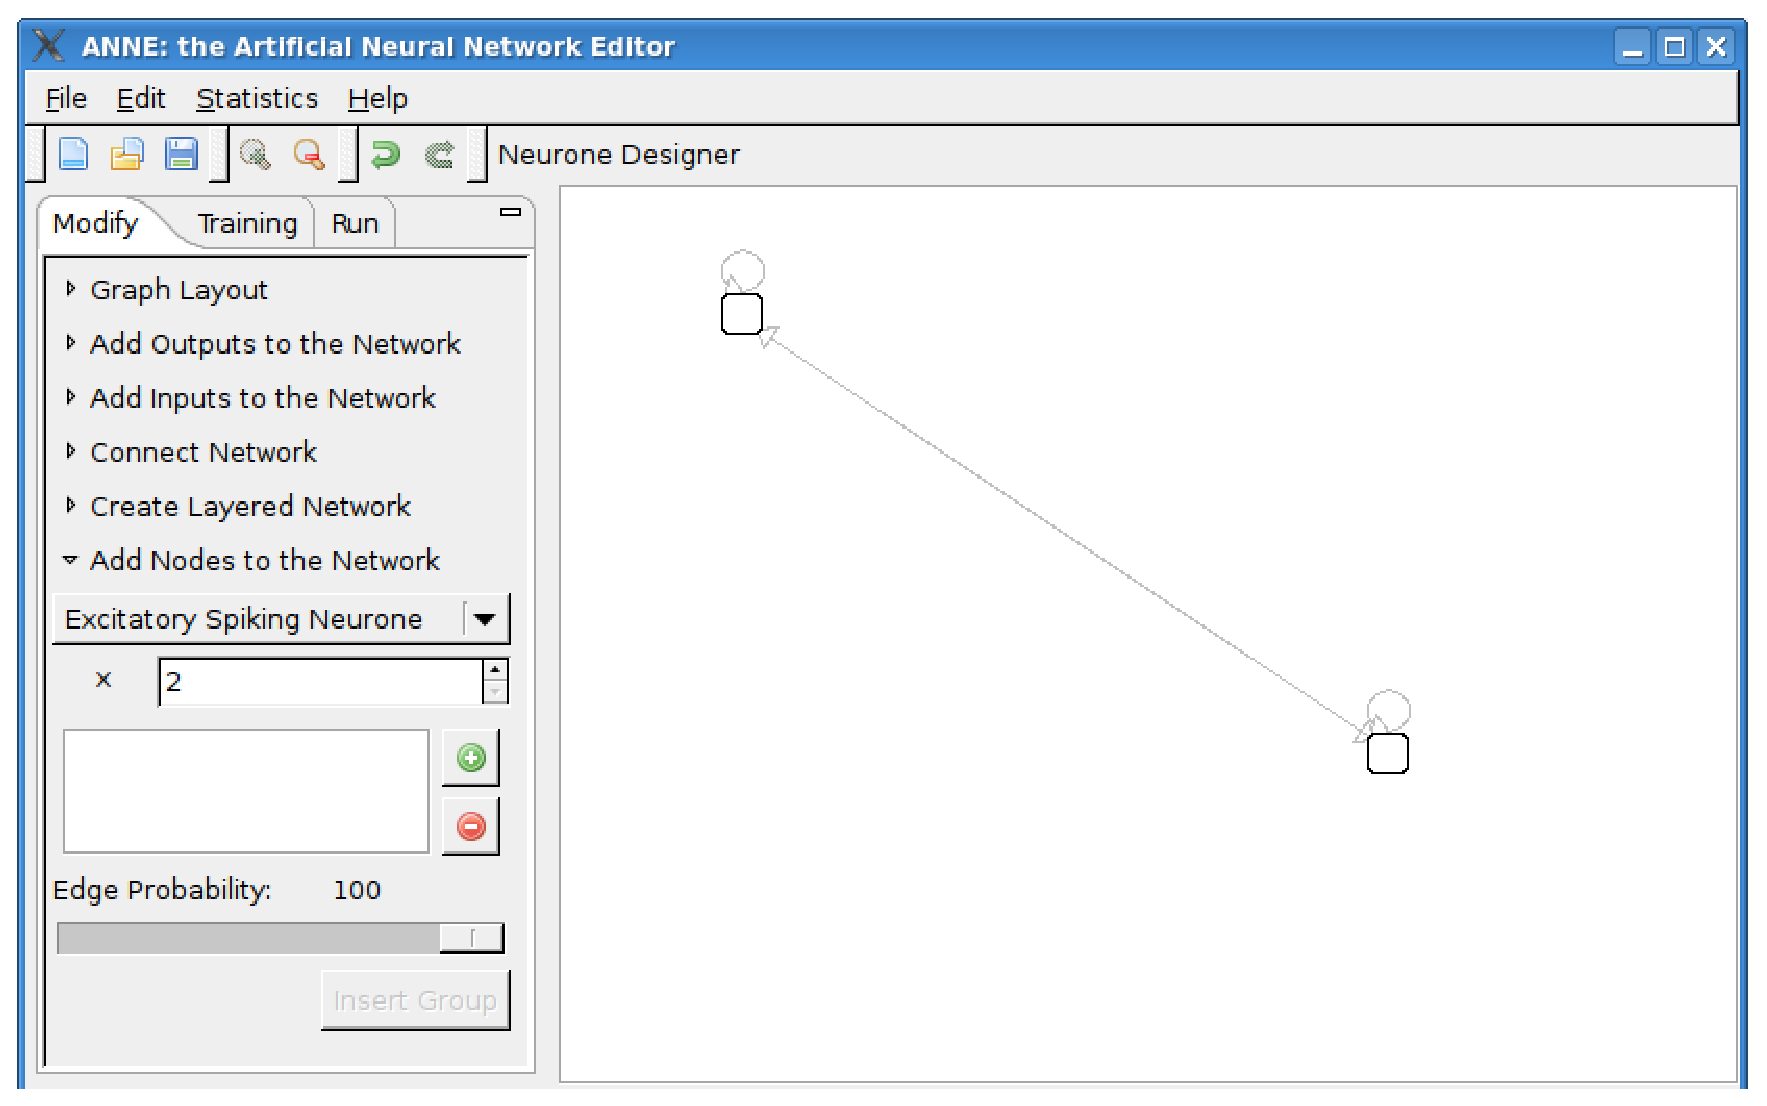
\includegraphics{examplenetlinux}
}
\caption{View of the example network in ANNE.}
\label{fig:persistence:egnet}
\end{figure*}
The example network used is one of two Excitatory Spiking Neurones with synapses linking them to each other and back on themselves (otherwise known as 100\% connectivity). A view of the network in the ANNE tool can be seen in Figure \ref{fig:persistence:egnet}.

It is easy to see that the TNS output is very light{}-weight but fairly hard to
interpret by a casual eye. By contrast, both the XML formats are very long but quite intuitive to read. It is also clear that the X3D output has lost a large amount of information on the neural network, which is the main reason why no importer for X3D could be written.

\begin{figure*}[t]
\centering
\scalebox{0.5}{
	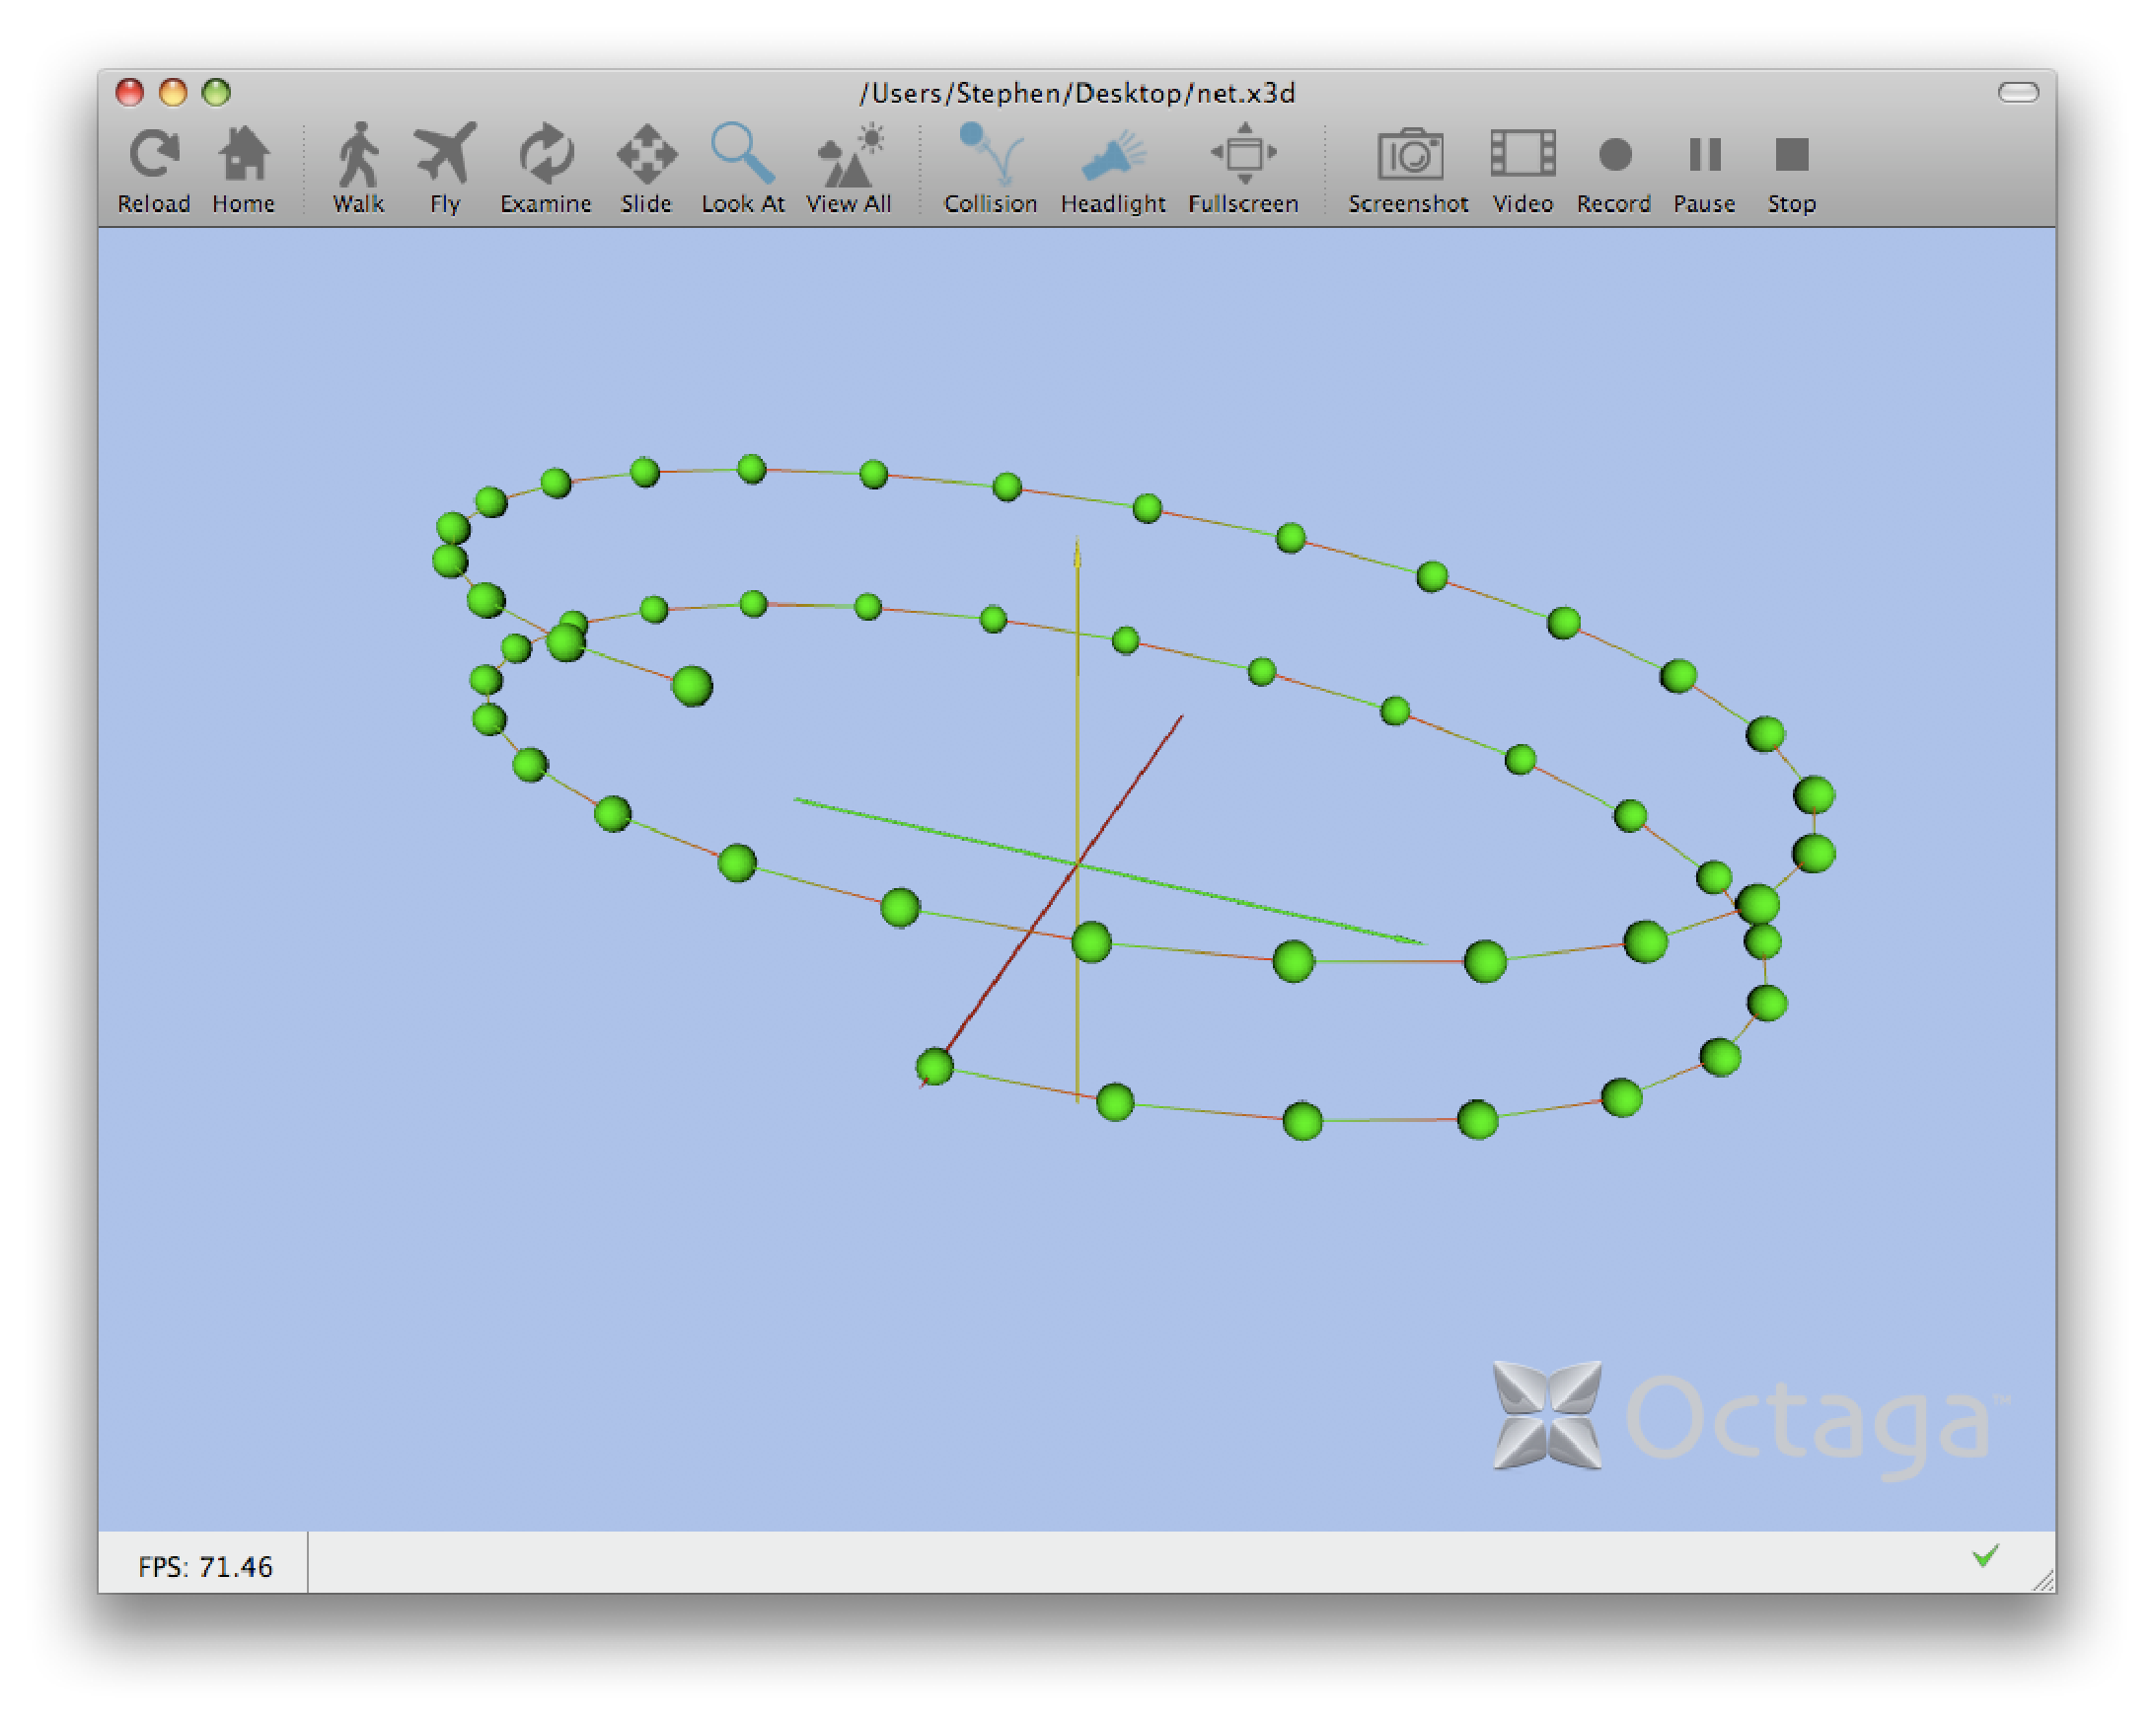
\includegraphics{octaga1}
}
\caption{View of a Network produced in ANNE displayed in Octaga}
\label{fig:persistence:octaga}
\end{figure*}
Finally, there is an example of the X3D output from ANNE being loaded into an X3D viewer called Octaga\cite{octaga}. This allows users to visualise their networks in a 3D space if they find that feature useful and demonstrates some of the  inter{}-application support within ANNE.
}

\subsection{Performance}
{
Networks were generated with the number of excitatory spiking neurones
as specified in the table and a 100\% connectivity probability,
networks were completely regenerated when changing between sizes.

\subsubsection{Benchmarking System}

\begin{itemize}
\item {
CPU  {--} 2.33GHz Core 2 Duo
}
\item {
Memory  {--} 2GB, 667MHz DDR2
}
\item {
Hard Disk {--} 160GB, 5,400rpm, 16MB cache
}
\item {
File System {--} Journaled HFS+
}
\item {
OS {--} Mac OS X 10.5.6
}
\end{itemize}

\begin{table}[t]
\centering
\begin{tabular}{|r || c | c | c | c |}
\hline
Size & Serialization & NeuroML (XML) & TNS & X3D \\
\hline
10 & 0.01 & 0.00 & 0.00 & 0.06 \\
50 & 0.19 & 0.06 & 0.00 & 0.48 \\
100 & 0.74 & 0.65 & 0.00 & 4.25 \\
500 & 16.97 & 5.43 & 4.27 & ? \\
1000 & 74.33 & 19.95 & 24.36 & ? \\
\hline
\end{tabular}
\caption{Performance Analysis - Save Execution Time}
\label{persistence:save}
\end{table}

\begin{table}[t]
\centering
\begin{tabular}{|r || c | c | c |}
\hline
Size & Serialization & NeuroML (XML) & TNS \\
\hline
10 & 0.06 & 0.15 & 0.05 \\
50 & 0.35 & 0.41 & 0.23 \\
100 & 1.01 & 0.71 & 0.69 \\
500 & 23.37 & 11.21 & 20.29 \\
1000 & 94.67 & 57.14 & 2091.74 \\
\hline
\end{tabular}
\caption{Performance Analysis - Load Execution Time}
\label{persistence:load}
\end{table}

\begin{table}[t]
\centering
\begin{tabular}{|r || c | c | c | c |}
\hline
Size & Serialization & NeuroML & TNS & X3D \\
\hline
10 & 10.93 & 37 & 13.86 & 21.02 \\
50 & 185.93 & 766.38 & 304.57 & 464.97 \\
100 & 716.7 & 2993.31 & 1202.03 & 1841.67 \\
500 & 17443.26 & 72470.61 & 32823.98 & ? \\
1000 & 69552.63 & 289717.38 & 122396.96 & ? \\
\hline
\end{tabular}
\caption{Performance Analysis - File Size (KB)}
\label{persistence:size}
\end{table}

%\textbf{\textit{Note:}} Graphs depicting the information in the above
%tables can be found in Appendix \ref{appendix:persistence:perf}.
\begin{figure}[t]
\centering
\scalebox{0.5}{
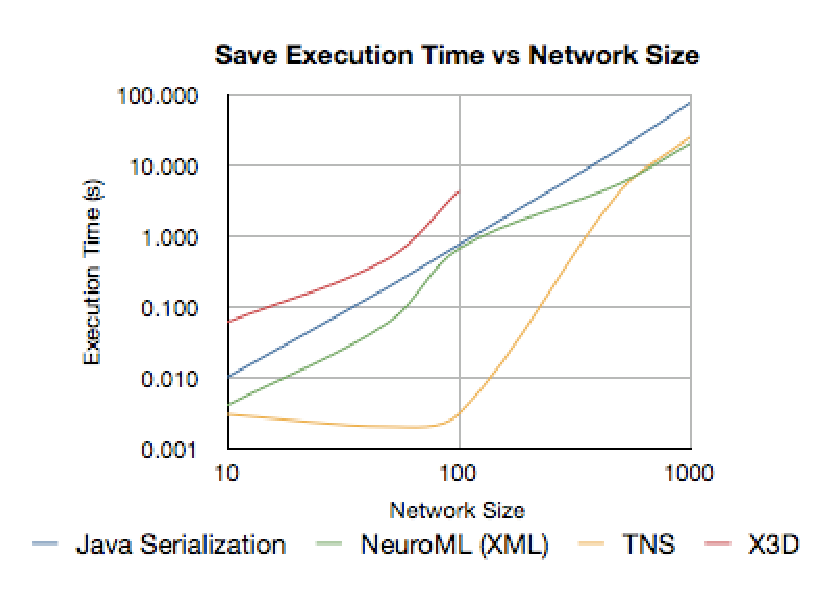
\includegraphics{persistence-save}
}
\caption{Performance Analysis Graphs: Saving}
\label{fig:persistence:perf:save}
\end{figure}

\begin{figure}[t]
\centering
\scalebox{0.5}{
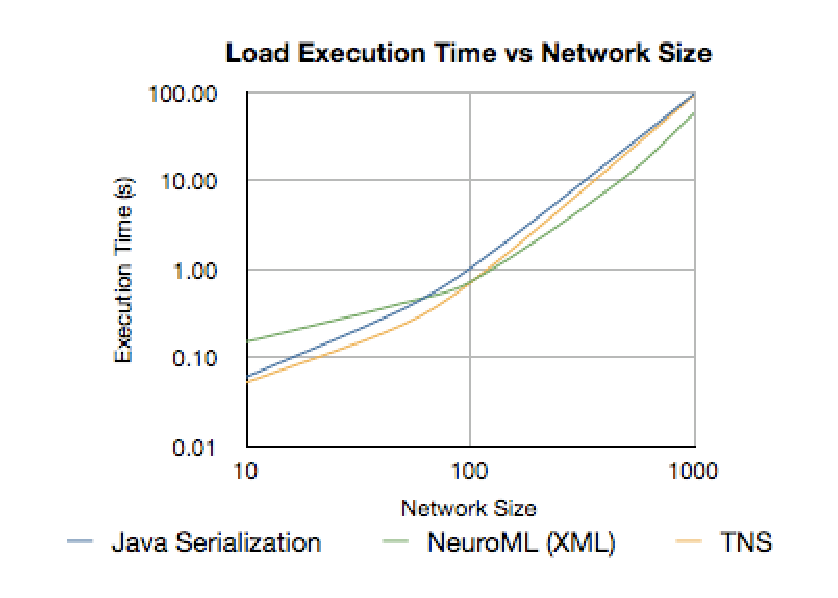
\includegraphics{persistence-load}
}
\caption{Performance Analysis Graphs: Loading}
\label{appendix:persistence:perf:load}
\end{figure}

\begin{figure}[t]
\centering
\scalebox{0.5}{
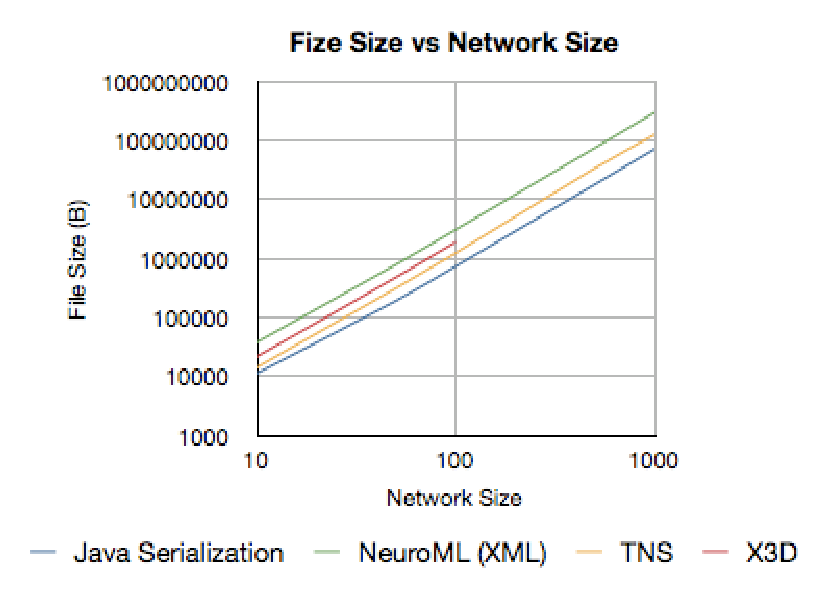
\includegraphics{persistence-size}
}
\caption{Performance Analysis Graphs: File Size}
\label{appendix:persistence:perf:size}
\end{figure}

\begin{figure}[t]
\centering
\scalebox{0.5}{
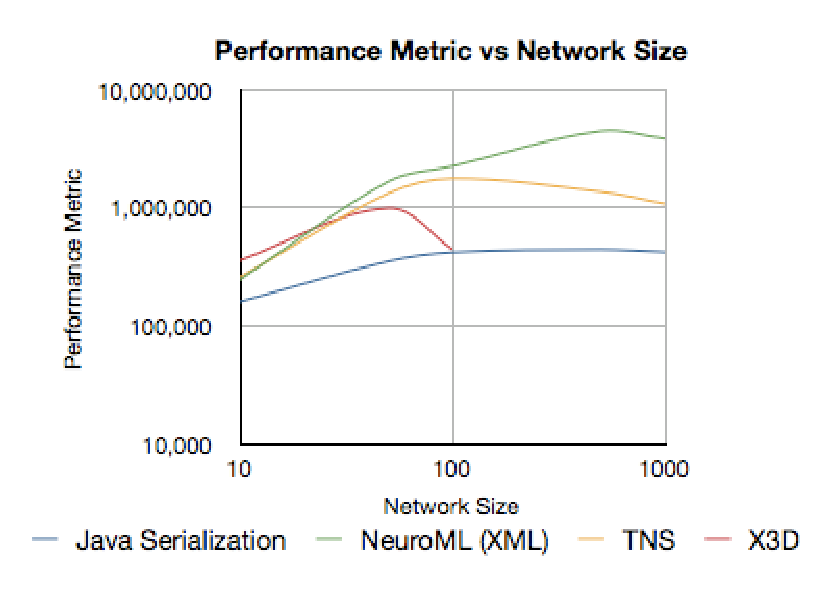
\includegraphics{persistence-metric}
}
\caption{Performance Analysis Graphs: Performance Metric}
\label{appendix:persistence:perf:metric}
\end{figure}

One clear observation from Tables \ref{persistence:save} and \ref{persistence:size} is that (as discussed previously) X3D failed to successfully produce any output on networks of size 500 and 1000. Also because of the implementation, nearly twice as much temporary storage is required during export, as the NeuroML XML document needs to first be produced so that it can then be read and can only be deleted after the transformation is complete. It is clear that a future release of the X3D plug{}-in should be implemented in a more efficient way.

NeuroML and Java Serialization grow linearly on a logarithmic graph for Save
and Loading time, suggesting that their execution time would predictably
grow with larger networks and would be easily estimated with network
sizes within the range of network sizes sampled. NeuroML generally
performs better than Java Serialization, especially with large networks,
however this is offset by NeuroML having a considerably larger
resulting file size than Serialization. With ever increasing network sizes this could start to cause problems {--} an option of compressing the output of the text based persistence methods could provide further flexibility to the user.

TNS demonstrates some interesting behaviour. Firstly, for networks below 100 neurones in size it requires significantly less time than all other persistence methods and requires no significant increase in time for sizes up to 100. After this it rises sharply but looks to begin levelling out to the same rate of increase as NeuroML and Serialization. This is potentially a result of the time taken in object allocation for the event stream. File sizes generated are significantly less than NeuroML (generally below half the size) but not as small as Serialization and the load time is competitive with that of serialization or NeuroML.

A performance metric was calculated that took into account the loading
and save times, as well as the file size generated, compared to the
network being persisted. The performance metric was as follows:

$\text{Performance Metric}=\frac{\text{Load Time}+\text{Save
Time}}{\text{File Size}}$

A lower value of this metric implies better peformance, as we can see from the graph which plots the metric against the network size that Java Serialization is the obvious performance winner. This was to be expected as even though it has a poor saving time it produces significantly smaller files than the other persistence methods and requires no extra time for loading. It is, however, important to temper this with the un-portability and readability / editability of its format. TNS and NeuroML look to be improving after reaching an initial storage overhead on network size, TNS beating NeuroML though because of the smaller file sizes produced. X3D was included for completeness, but no real information can be taken from the graph as X3D has no load time and could not complete all the tests.

It is worth noting that this performance analysis was only a fleeting look at persistence's real world observable performance and tests were run on production systems a single time, instead of multiple times to verify results. This means little more statistical analysis can be done on these results as there isn't the required information.
}

\subsection{Evaluation and Further Development}
{
The persistence module provides an easy and extensible way of implementing persistence plug{}-ins which can export the neural network model to storage or possibly another application. The initial persistence plug{}-ins provide the average user with a number of options for saving and exporting, with Java Serialization the recommend method for saving a small neural network for use with other instances of the ANNE application or incremental backup. NeuroML export is available for transferring your network to other applications and importing back from it.

Due to the pluggable nature of the system, further versions of a persistence option are not required to be released at the same time as the core framework, allowing for them to be worked on and released separately on a more rolling basis. New persistence options could be added later on if required for exporting to more specific or proprietary formats, thus allowing developers of other, potentially closed{}-source, applications to write their own plug{}-in to read their application output which could be distributed without having to reveal a specification of their file format. This ease of implementation would hopefully help ANNE become a more popular solution to model neural networks with.

Further development upon the persistence API could include:
\begin{itemize}
\item {
Further performance analysis of all the persistence plug{}-ins and optimizations of their code to improve execution time and memory usage.
}
\item {
The option for file compression after export would reduce the file sizes produced but obviously at the cost of execution time. There may be a point where a network reaches a certain size that it may be necessary to compress the output file; already with 1000 neurones NeuroML files reach 280MB, which even with current hard drive capacities is a large file. With the option to save to a compressed format, automatic decompression of files when loading would be required so that the new compressed files where supported. Perhaps a compression option that can back{}-end the serialisation to another service first before compressing its output could be a persistence plug{}-in to enable this without requiring modifications to the existing code{}-base.
}
\item {
ANNE's current X3D implementation is incapable of exporting large networks because of the problems using XSL transformations on large XML documents. A bespoke plug{}-in which is not dependent on the NeuroML plug{}-in would probably be a better alternative implementation. Furthermore, this would reduce the amount of storage required for export as currently an XML must be produced before being read again and then deleted.
}
\item {
Further persistence options such as exporting to other neural network modelling standards and file formats, for example the previously mentioned PyNN as well as Matlab's Neural Network tool.
}
\item {
An auto{}-save feature would be a useful addition, permitting users not to have to remember to periodically save their work, in case of mistake or system failure. It could be implemented by creating another thread which sleeps for the auto{}-save time period and then fires the save manager off to save to a temporary location before sleeping again. ANNE could then poll this location for auto-save files in the event of a crash and load a network's state from the previous session.
}
\end{itemize}
}

\section{User Interface}
\subsection{Overview}
{
ANNE's user interface aims to be as intuitive as possible, yet still allow efficient execution of complex tasks. It is highly modular, and many different aspects of functionality can be added as plugins.
}
\subsection{Design}
\subsubsection{GUI Framework}
{
When looking for a GUI framework to use for our application, there were certain requirements that needed to be met. The framework had to allow us to easily draw graph objects, as well as move them around the graph by dragging and dropping. This graph also had to be expandable and easy to navigate via scrolling. Several frameworks were tested by implementing simple neural networks in code, and checking whether or not it would be simple to fulfil our requirements.

When starting to look at ways to implement the GUI in Java, we first looked at SWT\cite{lib:swt}. SWT has several advantages; it is well documented, cross platform and has plenty of on-line support. After experimenting with SWT we found that while it was suitable for our main GUI layout and menus, it did not meet our requirements for displaying graphs. Drawing each neuron and synapse as a separate SWT canvas gave unusable result as each canvas must be rectangular, and there is no support for transparent backgrounds. This meant that if synapses overlapped, the background of one would obscure the other. The only other option using pure SWT would be to write an entire graph visualisation package that draws its results onto a single canvas, which we deemed to be too time-consuming.

\begin{figure}[t]
\centering
\scalebox{0.4}{
	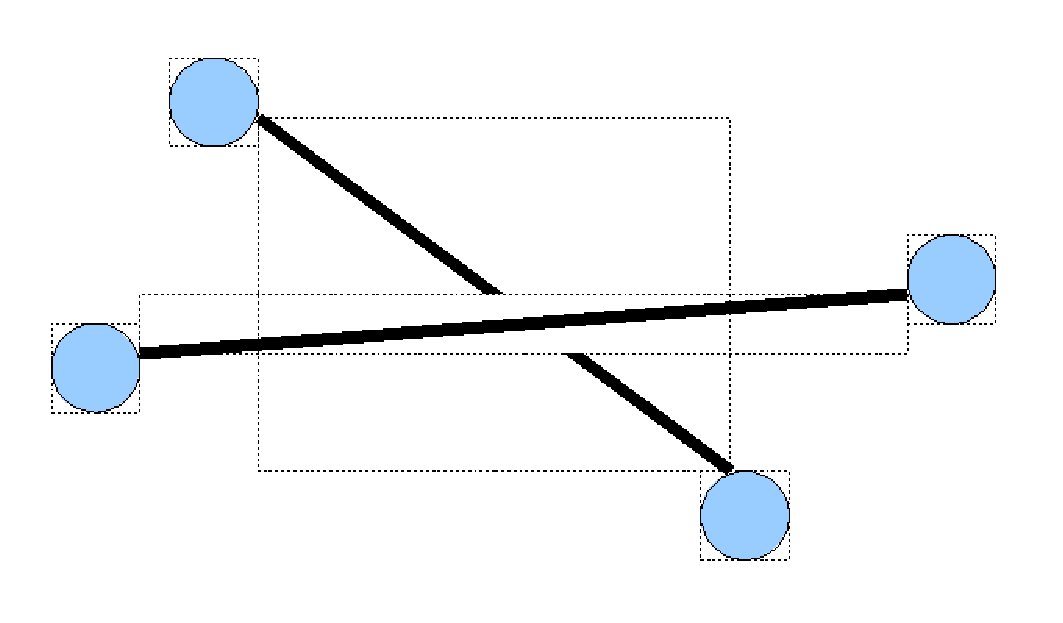
\includegraphics{NNDraw2d}
}
\caption{The Problem With Draw2d}
\label{fig:ui:draw2d}
\end{figure}

Our next candidate was the Draw2D framework\cite{lib:draw2d}, which runs inside an SWT canvas and displays graph nodes and edges. This is a subset of the Graph Editing Framework \cite{lib:gef}, which is a heavyweight framework for creating graphical editor software. Although GEF included graph editing functionality, it was too inflexible for our plugin-oriented architecture and multi-layered networks. Draw2D allowed us to have transparent backgrounds on graph objects, but there was still no native support for scrolling, dragging and dropping, or other common graph functions. The lack of clear documentation for the framework caused us to run into problems implementing these features, such as irremovable artefacts appearing whenever the main canvas was scrolled.

We then moved onto Zest\cite{lib:zest}. Zest is a larger subset GEF that builds on top of Draw2D and includes the common graph functions described above. This was ideal for our program since it did everything we required, so we decided to use it despite its poor documentation.
}
\subsubsection{GUI Layout}
{
While designing the layout of the application, we took many things into consideration. Our main focus was making the application as easy to use as possible without limiting functionality. The design of the high-level GUI layout was discussed at length towards the start of our project, before we agreed on a single design. We have all had experience programming in Integrated Development Environments (IDEs) such as Eclipse, and felt that many features common to these programs would cross over to creating and testing large-scale artificial neural networks.

The final layout we decided on is split into panels, in a similar manner to existing IDEs. The top panel contains a menu and tool bar, the left panel contains a sidebar for all network editing operations, the bottom panel is a ticker containing important logging information, and the main panel displays a view of the neural network. Each of these panels can be grabbed and resized, as is standard for applications of this type, and their contents can easily be extended using plugins.

We decided to split the sidebar into three sections corresponding to the three ways in which people interact with neural networks: modify, train and run. The modify tab contains plugins related to editing the structure of the network such as adding groups of neurones, adding special inputs and outputs, and connecting existing subnetworks. The training tab lets people select a training algorithm, set parameters and train a network. Finally, the run tab lets users run simulations on a network.
}
\subsubsection{Neural Network Visualisation}
{
One of the main issues inherent in building a system of this type is the difficulty involved in viewing and navigating huge networks. A simple graphical solution is to display each neurone and synapse in the neural network as a single graph, which can be scrolled vertically and horizontally as needed. This is fine for networks containing a few dozen nodes and synapses, but finding specific locations in larger graphs can become time-consuming.

A proposed fix for this problem was to let users quickly 'bookmark' frequently-accessed sets of neurones, which could then be viewed using keyboard hotkeys or a menu. This technique was inspired by the interfaces of various Real-Time Strategy computer games, in which users can place units into groups and automatically snap the view to any of their locations, even when they are spread throughout a large battlefield that would be slow to navigate otherwise.

This was more useful than the first implementation, but still had its problems. Users must remember which hotkey relates to which set of neurones, and make sure to add and remove neurones from sets as necessary. Navigating to neurones that are not bookmarked is no easier than before, so a large number of groups must be created if several locations in a network must be accessed often.

Allowing the user to zoom in and out of the whole network is a far more efficient solution from a user perspective, as it enables quick navigation to any section of the graph without having to mentally maintain a list of bookmarks. However, large networks often consist of dense groups of neurones that are highly connected by a huge number of synapses. Even with zooming, the amount of visual clutter present when viewing each separate neurone and synapse makes the task of navigating densely-connected networks far from easy.

\begin{figure}[t]
\centering
\scalebox{0.2}{
	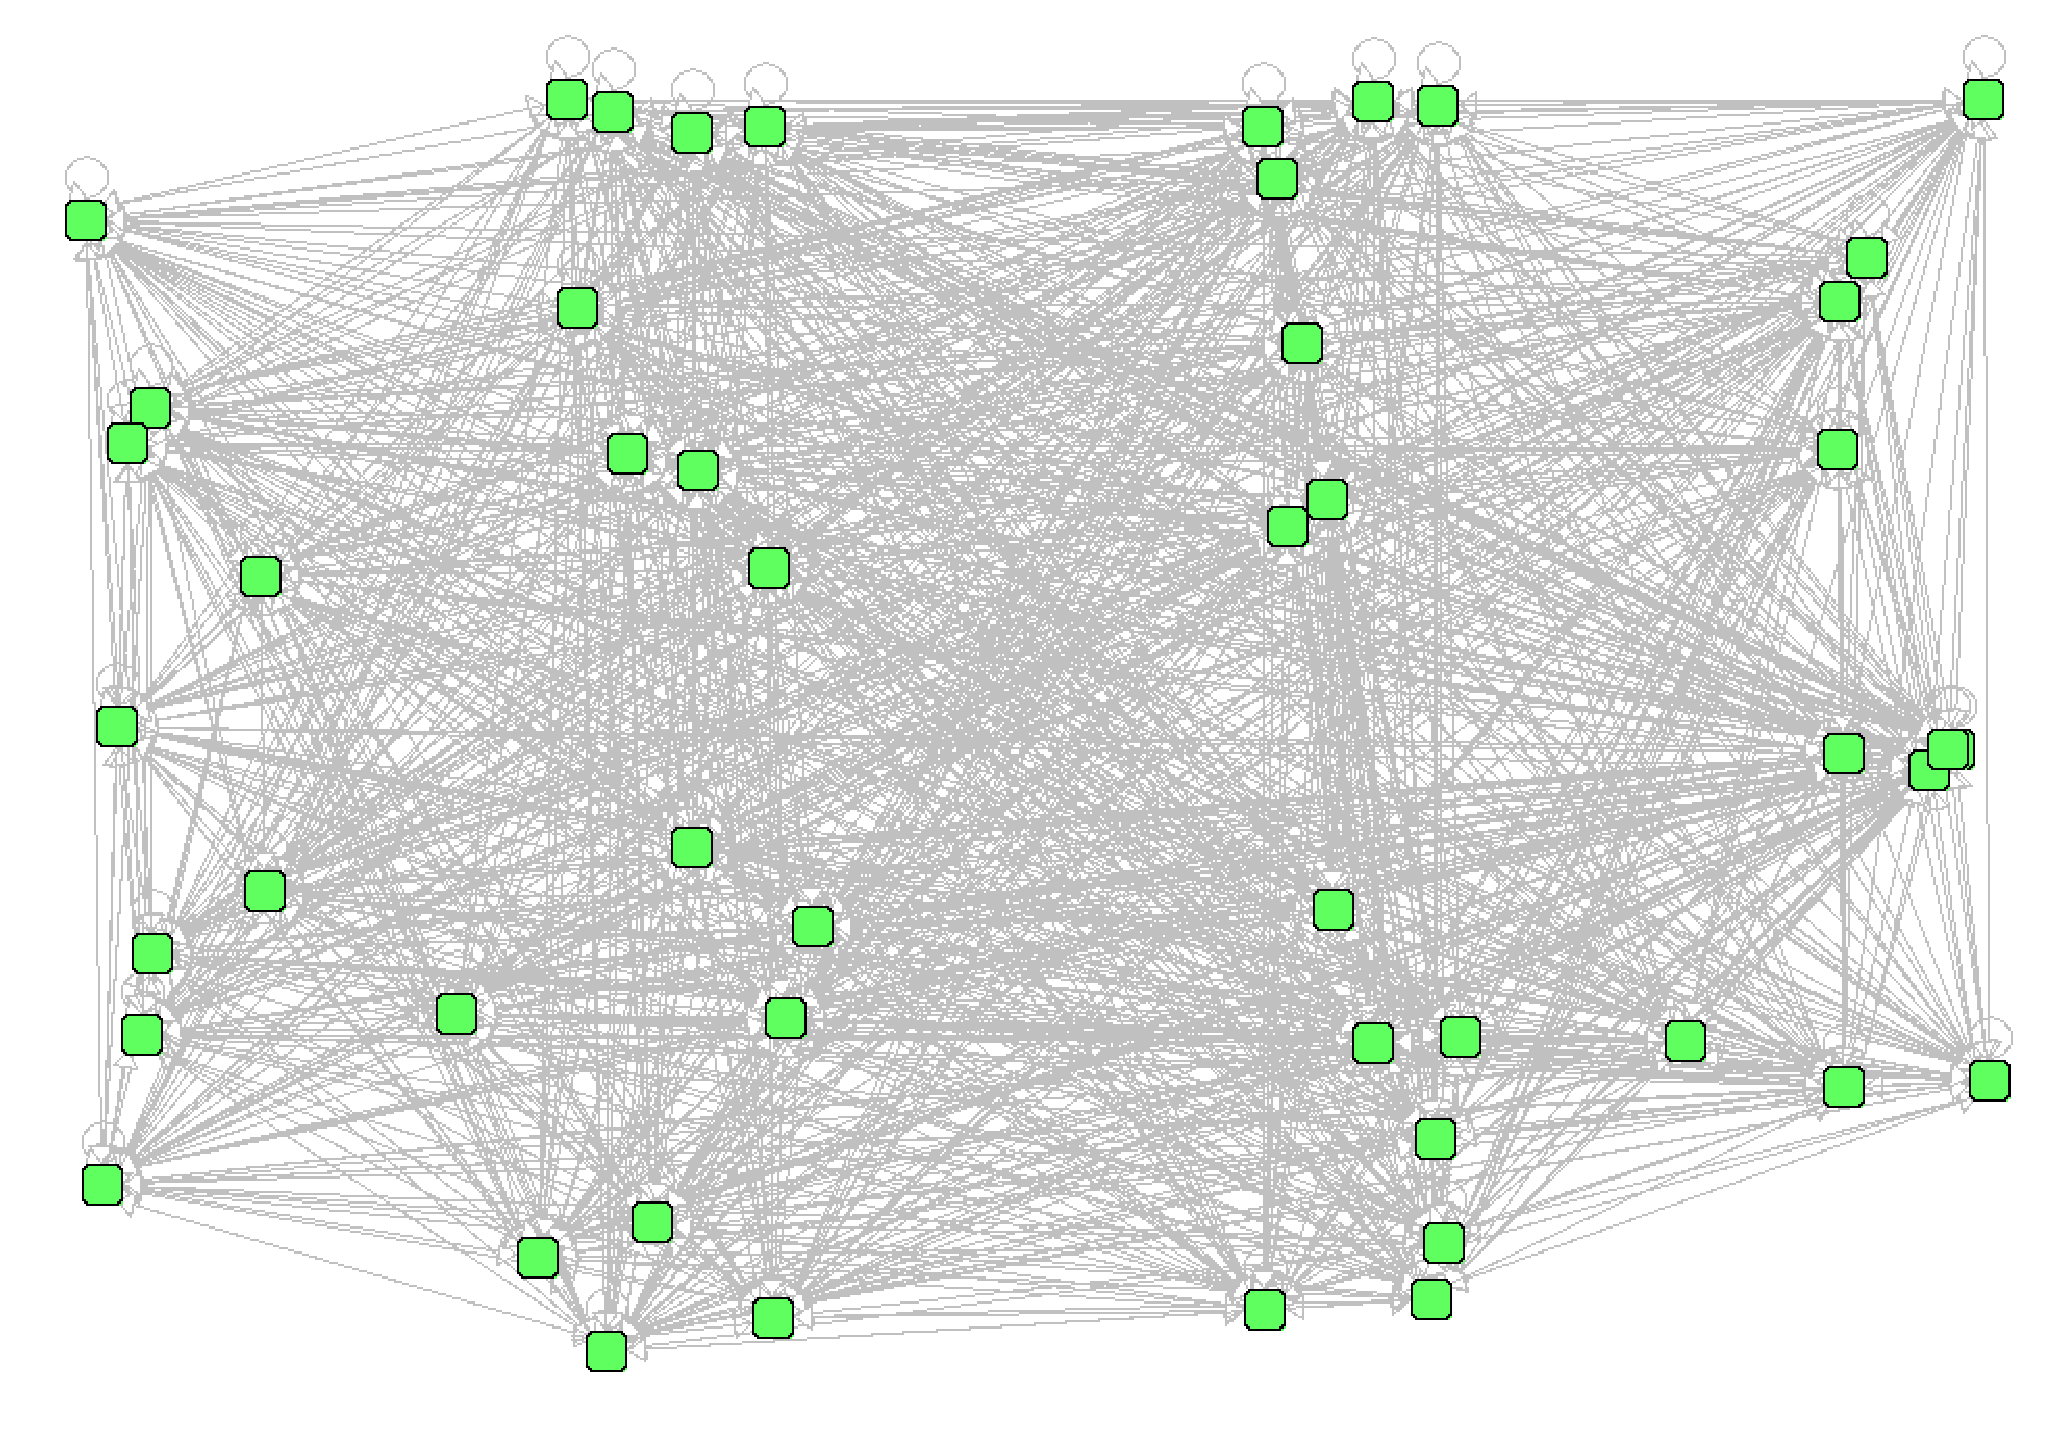
\includegraphics{lotsOfNeurones}
}
\caption{A group of 50 densely-connected neurones}
\label{fig:ui:lotsofneurones}
\end{figure}

This clutter (Figure \ref{fig:ui:lotsofneurones}) was reduced by grouping sets of neurones and synapses within a network into single graph entities, then consolidating all synapses between a pair of groups into a single bridge. Our original plan was for these groups to be created and destroyed intelligently by the system as a user zoomed in and out, but the algorithm to do so would be difficult to design. The program must support many existing types of network and be extensible so that many other types can be used in the future, but these types have different notions of how groups should be organised. Implementing several such algorithms for different network configurations would be time-consuming in itself, and a programmer extending the system to support a new network type would have to write another of these neurone grouping methods.

To aid ease of navigation and customisability as much as possible without compromising ease of extension, we instead let users manually create and edit these internal groups of neurones and synapses in whichever way makes the most sense for their network. These groups can be nested within each other, and navigation consists of zooming into and out of the tree-like hierarchy of groups as needed. Each of these groups in our system is itself defined as a neural network, which makes it trivial to import subnetworks into other networks and fulfil our requirement that modular networks are supported.

A few additional features were added to minimise the time it takes to obtain information from a neural network. Hovering the mouse over a subnetwork or a network bridge displays a tooltip containing a summary of its contents, and clicking the arrow by a subnetwork's name expands it to show the number of components it contains. We found this minimised the time it took to check these values, without the unacceptable visual clutter that would have resulted from displaying all of this data at all times.

\begin{figure*}[t]
\centering
\scalebox{0.4}{
	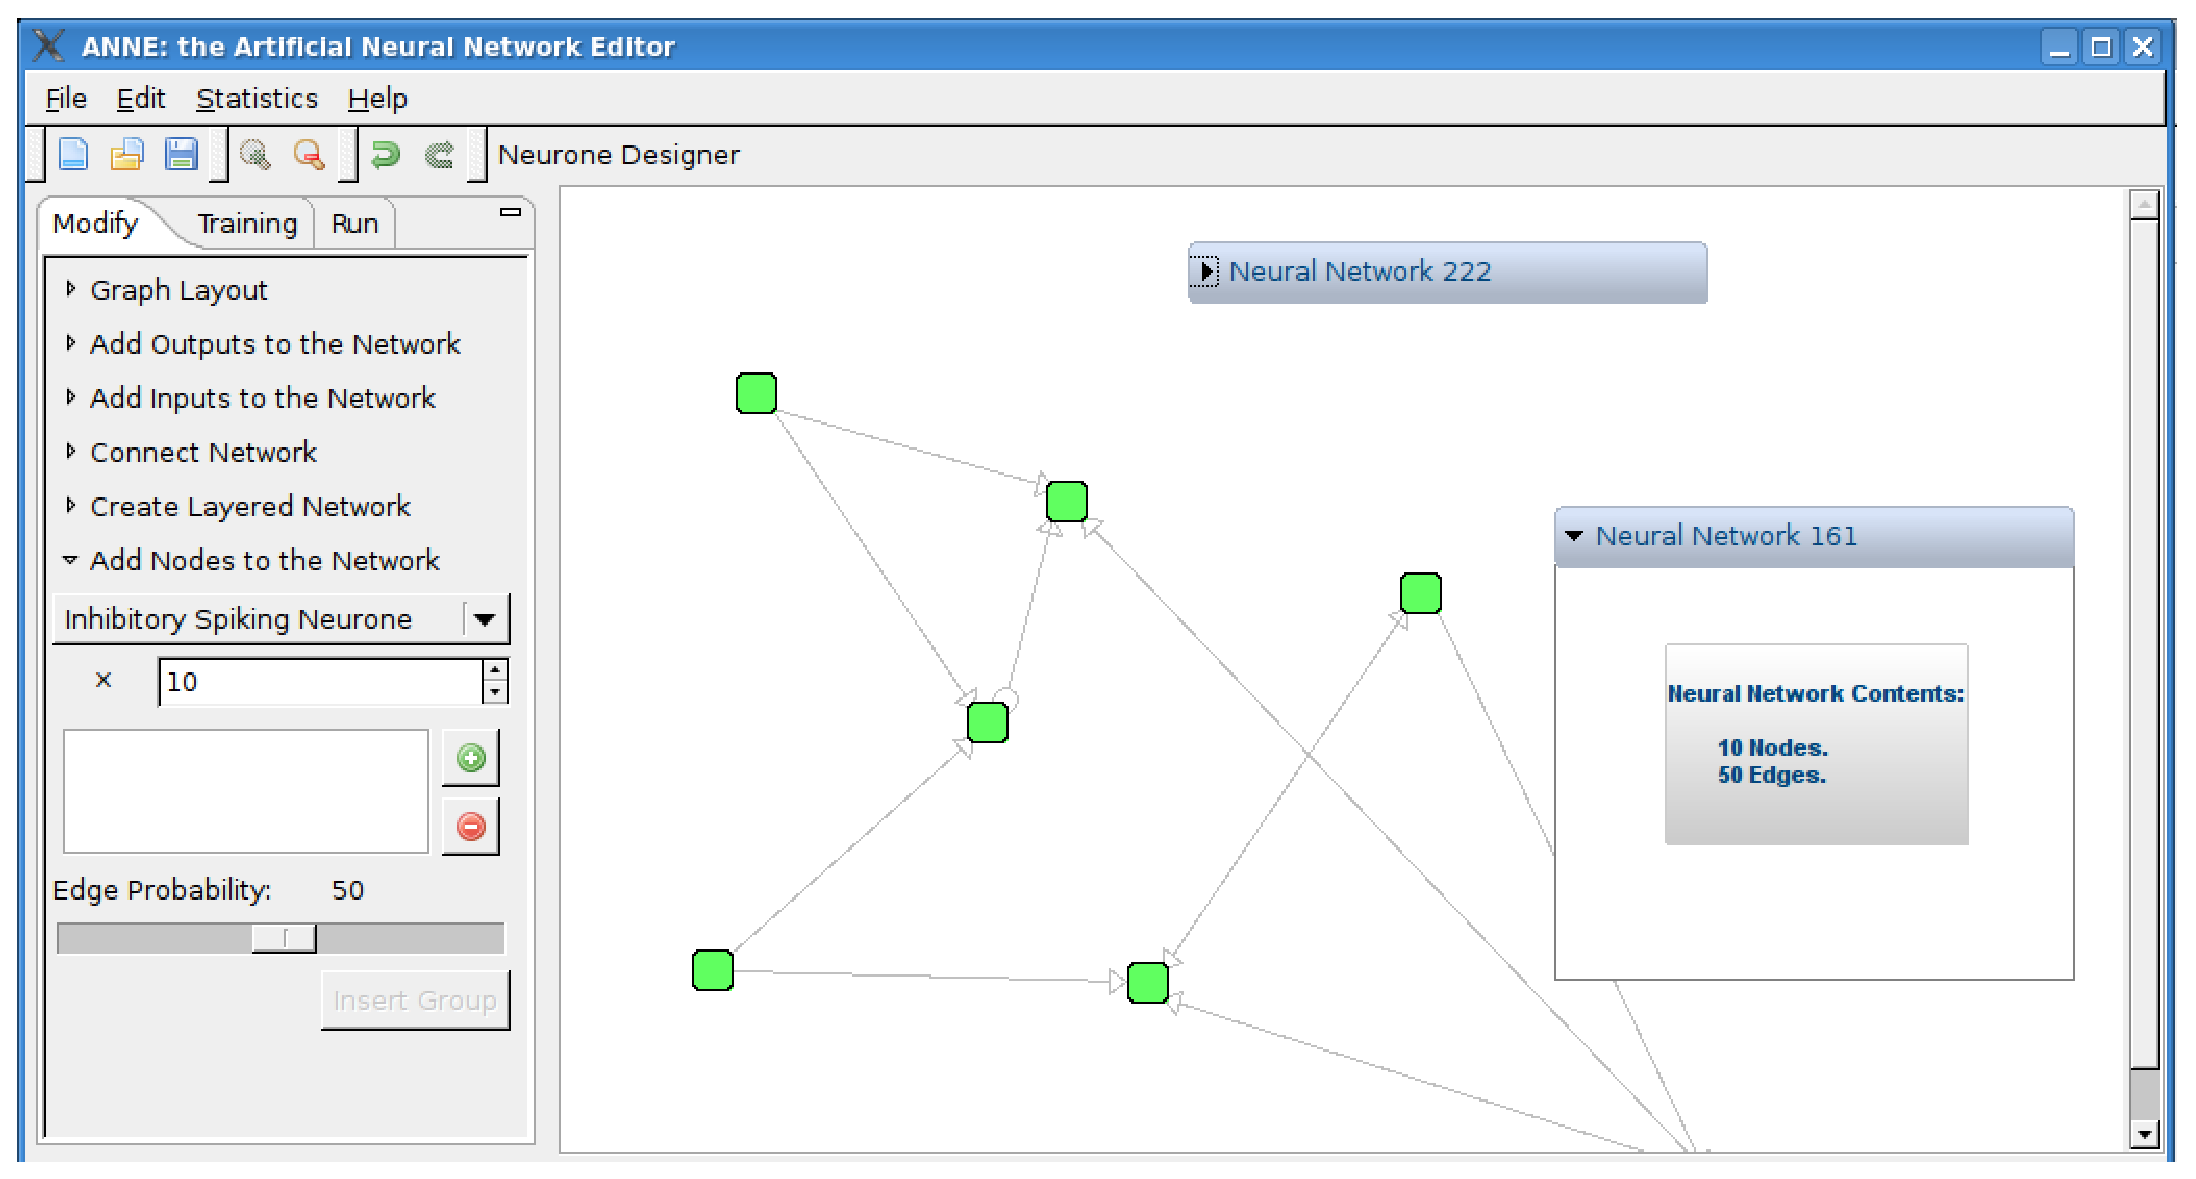
\includegraphics{layeredNetwork}
}
\caption{Layered Networks}
\label{fig:ui:layered}
\end{figure*}
Figure \ref{fig:ui:layered} shows a layered network containing 3 subnetworks connected by 2 network bridges. One subnetwork is expanded, and the selected network bridge's tooltip is visible.

In addition to neural network's layout, the user must also be able to efficiently view its state. Individual neurones and synapses, much like subnetworks and network bridges, contain tooltips showing the values of their parameters. Also, as is standard for diagrams of neural networks, synapses from inhibitory neurones use circle arrowheads instead of the usual triangles. We felt this gives the user as much information as possible without cluttering large networks.

\begin{figure}[t]
\centering
\scalebox{0.5}{
	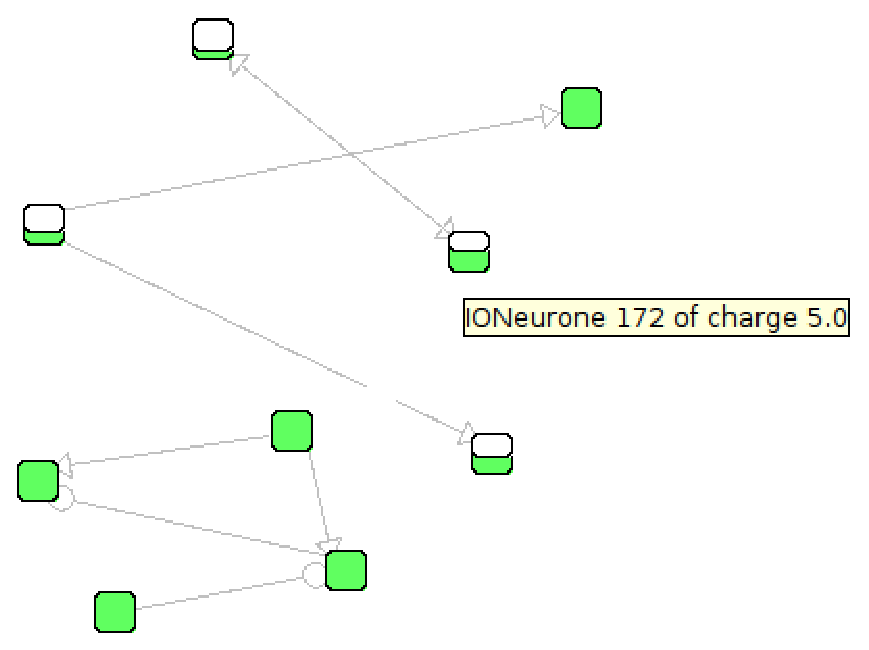
\includegraphics{specialGraphElements}
}
\caption{Circle and triangle arrowheads, charge overlays and a visible tooltip}
\label{fig:ui:special}
\end{figure}
}

\subsection{Implementation}

\subsubsection{User Interface Core}
{
Our Graphical User Interface builds on top of ANNE's framework and graph packages without any back-references, in such a way that the entire GUI can be replaced or removed altogether without having to change any code in those packages.

The core features that must be implemented by any user interface are encapsulated in the coreui package, and the InterfaceManager class contains the most basic of these features. Any interface manager must be able to import, edit and export neural networks, handle saving to different file locations and hold a CommandControl object. It also contains an instance of InteractionUtils, which is a class containing common neural network functionality which will be useful to most user interfaces. This includes running and pausing networks, creating sets of nodes, finding the parent networks of nodes, and bifurcating networks.

For user interfaces that support zooming, the ZoomingInterfaceManager interface is available. Different zoom levels are represented as a stack of NeuralNetwork references, with the root network at the base and the current view as the head. A stack containing the IDs of each zoom level is also available, which can be efficiently accessed by anything that needs to know the path from the root network to the current view.
}
\subsubsection{GUI Manager}
{
The InterfaceManager used by our GUI is the GUIManager, which draws the current view of the neural network onto an SWT canvas using the Zest framework. A graph model is imported into the view using two Transformers, which convert Node and Edge types from the model into the appropriate GUI graph elements. If a synapse to or from an external subnetwork is passed into the GUIManager, an appropriate source or sink node is created and the edge is attached.

These entities are arranged on-screen using any chosen Zest layout, with our CachingLayout working underneath to add common functionality. Source and sink nodes are automatically arranged down the left and right sides of the screen respectively, and all node locations are persisted after zooming in and out. This lets users freely zoom in and out of a multi-layered neural network without its on-screen layout constantly changing.
}
\subsubsection{Graph Visualisation}
{
Each of the entities that comprises a neural network must be represented in the main view panel. These components are neurones, synapses, neural networks, and the network bridges that connect these networks. Each of these objects can be dragged and dropped, and they highlight and de-highlight appropriately when selected and deselected.

Neurones are represented in the user interface as GUINode objects. These extend Zest GraphNodes and are drawn as small rounded rectangles, with a white overlay showing the neurone's current level of charge. This overlay begins at the top of the node, and grows to cover more of it as the charge decresases. If a neurone has no charge at all, this overlay covers the entire node. This gives the appearance of the node background colour being the colour of the charge, and the overlay colour being the 'background' colour.

Different types of network inputs and outputs are implemented as subclasses of InputNode and OutputNode, and are kept in the \\gui.graph.ionodes package. Each type of node implements the \\Runnable interface, and contains the code needed to initialise any graphical elements used by itself such as SWT shells. The following types of IO node are currently implemented in ANNE:
\newpage
\begin{itemize}
\item {
DATInputNode, which takes a DAT input file and creates a subnetwork containing the appropriate neurones.
}
\item {
PunchingInputNode, which creates the given number of neurones and lets the user control their charge via sliders in an SWT shell. Each neurone's charge can also be disabled and enabled by a button above its slider.
}
\item {
ValueListingOutputNode, which creates a subnetwork containing the given number of neurones and displays their values in an SWT shell.
}
\end{itemize}

\begin{figure}[t]
\centering
\scalebox{0.5}{
	\includegraphics{configureChargeNodes}
}
\caption{Punching Input Nodes}
\label{fig:ui:configcharge}
\end{figure}

\begin{figure}[t]
\centering
\scalebox{0.5}{
	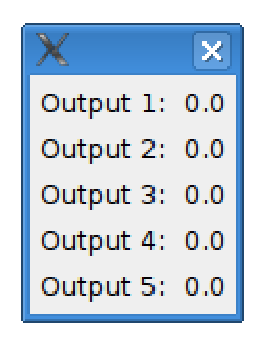
\includegraphics{ValueListing}
}
\caption{Value Listing Output}
\label{fig:ui:valuelisting}
\end{figure}

Synapses and network bridges are depicted as GUIEdge and GUIBridge objects respectively. These are both implemented as zest connectors, but GUIBridges are much thicker than GUIEdges to represent the fact that they contain several edges going from one neural network to another. 

GUINetwork objects represent the neural networks layered inside other networks. These are implemented as Zest GraphContainer objects, which can be expanded to show their contents. The 'contents' shown by a GUINetwork is a single Zest graph node, labelled with a text summary of the number of nodes and edges it contains. This is more readable than showing the entire GUINetwork's contents as a small graph, and also uses far less memory.

\begin{figure*}[t]
\centering
\scalebox{0.4}{
	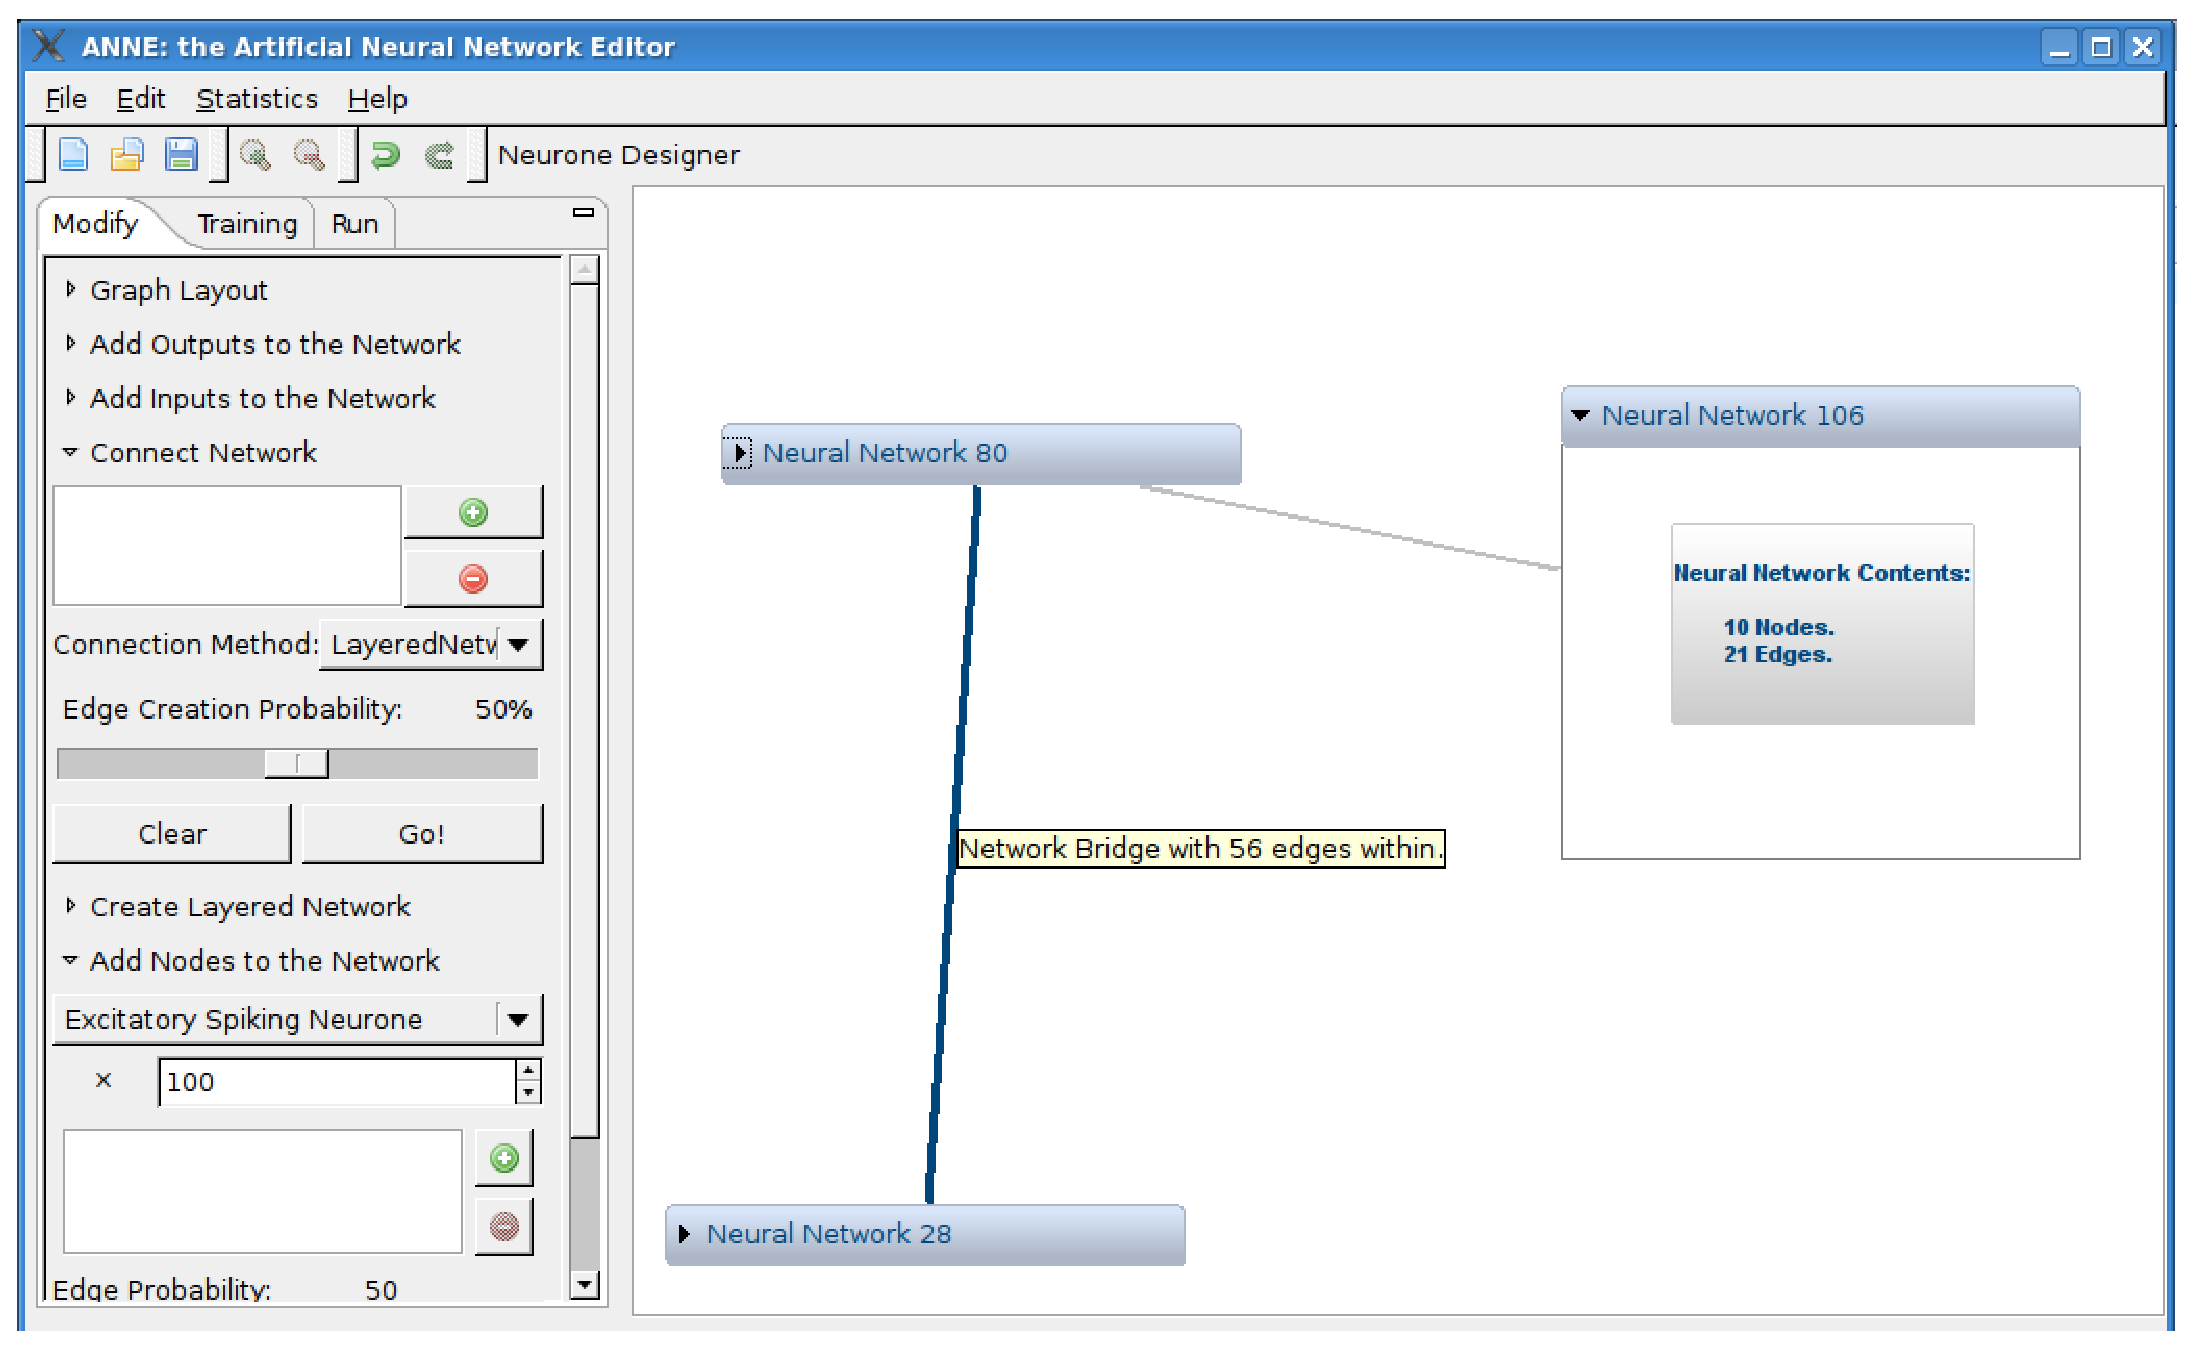
\includegraphics{layeredNetworkTooltip}
}
\caption{GUINetworks connected via GUIBridges, including a Dropdown Box}
\label{fig:ui:networkconn}
\end{figure*}

Our GUI contains an additional type of GraphNode, which is not included in the internal model of the neural network. This type of purely decorational node is the GUIAnchor. These nodes are shown as small black squares, and they represent connections to and from external subnetworks. These nodes are divided into sources and sinks, which define incoming and outgoing connections respectively. As GUIAnchors are not stored in the internal model, they are created and destroyed after each zoom action and are laid out automatically instead of having their positions persisted.
\begin{figure*}[t]
\centering
\scalebox{0.4}{
	\includegraphics{Connectingneurones3}
}
\caption{GUIAnchors in a Neural Network}
\label{fig:ui:guianchor}
\end{figure*}
}
\subsubsection{Top Panel}
{
The top panel of our user interface consists of the tool bar and the menu, both of which are implemented using SWT.

The tool bar is constructed using a CoolBar from the SWT library (Reference SWT). A CoolBar contains several ToolBars, each of which represents a group of buttons. These buttons are simply SWT ToolItems. Users can drag and resize each ToolBar, as is common for applications of this type.

Like the rest of our user interface, the tool bar is pluggable. This lets users add new ToolBars or ToolItems without having to edit the existing GUI code. The ToolItems currently included in the CoolBar are (sorted by ToolBar):
\newpage
\begin{itemize}
\item{
New, Open and Save
}
\item{
Zoom In and Zoom Out
}
\item{
Undo and Redo
}
\end{itemize}

\begin{figure}[t]
\centering
\scalebox{0.5}{
	
\includegraphics{ToolbarAllHighlighted}
}
\caption{Tool bar with all buttons highlighted}
\label{fig:ui:toolbarall}
\end{figure}

The individual buttons in the ToolBar can also handle incoming events, and react accordingly. The main use for this feature is to tell buttons to enable or disable themselves after appropriate events, such as the undo button checking the size of the undo stack after each CommandEvent and disabling itself if it is empty.

\begin{figure}[t]
\centering
\scalebox{0.5}{
	\includegraphics{ToolbarSomeHighlighted}
}
\caption{Tool bar with some buttons highlighted}
\label{fig:ui:toolbarsome}
\end{figure}

The icon set used for the tool bar is the Silk Icon set\cite{famfamfam}. These were picked because they are widely used icons that clearly convey their meanings the user.

The menu uses an SWT Menu object, and is similarly pluggable. Existing plugins contain functionality for opening, loading and saving files, undoing and redoing actions, starting and stopping output plots, and more.

The sidebar is an SWT CTabFolder, and automatically loads plugins in a similar manner to the other panels. The 'train' and 'run' tabs are implemented as TrainingPanel and RunPanel, and the modify tab populates itself with any given NetworkModifier plugins.

The bottom panel is implemented as an SWT container, containing a scrolling text appender. This appender receives incoming log messages from Log4j, formats them, and scrolls the pane so the most recent messages stay onscreen.
}
\subsubsection{Commands and Plugins}
{
Undoable actions within the user interface are implemented to be Commands. These actions currently comprise adding and removing different types of graph items from the network, whilst ensuring that no inconsistencies occur and that the view never tries to display a network that has been removed. To ensure extensibility these commands are invoked by plugins that are implemented either as items to be added to existing menus or toolbars, or as Listeners.

Listeners are in the gui.graph.listener package, and work by listening for events such as mouse clicks or keypresses by extending MousePlugin and KeyboardPlugin respectively. Actions that are implemented as GUI plugins include:
\begin{itemize}
\item{
Selecting several graph elements by dragging a box around them with the mouse, as ElasticBandSelectionListener
}
\item{
Creating synapses by selecting a node and Ctrl-clicking another node (or command-click on Mac), as EdgeBuildingListener
}
\item{
Deleting all selected graph items with the 'delete' key, as MassDeletionListener
}
\item{
Sending an event to inform the zoom buttons on the toolbar of changes in selection, as ZoomListener
}
\end{itemize}

Different statistical methods for connecting networks are also implemented as plugins, based on the base NetworkConnector class. A list of Nodes is passed to these plugins' connect() methods, and a set of edges to be added to the neural network are returned. Our currently implemented network connectors are:
\begin{itemize}
\item{
Simple random connector, which creates edges at random between the given nodes
}
\item{
Small worlds connector, which connects groups of nodes by re-routing existing edges, on Murray Shanahan's research (at the time of writing, un{}-published)
}
\item{
Layered network connector, which creates unidirectional network bridges on a path through the selected subnetworks.
}
\end{itemize}

These plugins are automatically loaded into the Modify tab of the sidebar, and can be selected via a drop-down box.
}
\subsubsection{Plots and Statisticians}
{
The Event management system discussed in the Framework section makes it feasible to implement a generic means for exporting run{}-time data from the system. The primary data identified to be of interest to users is that of neurone firing patterns. As a result, three standard statisticians were implemented to output this data; one for real-time navigable raster plots, and two to output files (comma separated values, and a Matlab matrix with associated plot). All of these statisticians are built atop the {\textit{NumericalStatisticin}} interface previously discussed.

\begin{figure}[t]
\centering
\scalebox{0.8}{
	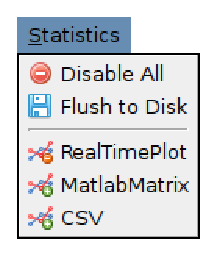
\includegraphics{statisticsmenu}
}
\caption{The Statistics Menu {--} RealTimePlot Enabled}
\label{fig:ui:statsmenu}
\end{figure}

To achieve this in the GUI, a statistician such as these may have a GUI configurator loaded. This presents itself as an option in the "Statistics" menu (Figure \ref{fig:ui:statsmenu}), to enable and disable the selected statistician. When enabled, the configurator is requested to configure its {\textit{EventHandler}}, and report the classes it is to be registered for. In this way, the statistician developer can write a minimum of code. For example, the CSV and Matlab Matrix statistician configurators simply prompt the user for a location to save their output file. They then write this data to disk either when the "Flush Data to Disk" option is selected, or when the statistician is disabled.

\begin{figure}[t]
\centering
\scalebox{0.5}{
	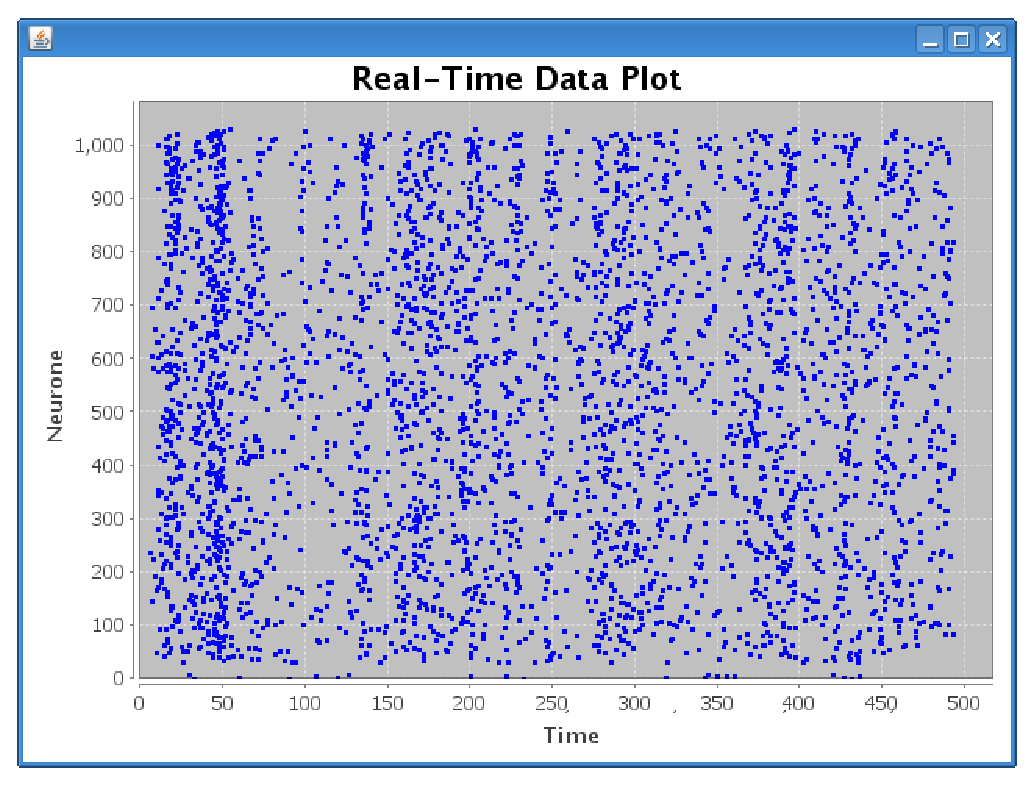
\includegraphics{realtimeplot}
}
\caption{RealTimePlot on a spiking neurone network exhibiting gamma wave patterns}
\label{fig:ui:realtimeplot}
\end{figure}
The RealTimePlot (Figure \ref{fig:ui:realtimeplot}) displays node firing patterns as a raster plot, updating in real{}-time as the network runs. It also supports navigation of the plot, including zooming and x{}-axis panning for browsing longer network runs.
}
\subsection{Evaluation and Further Development}
{
The GUI provides a clean interface for creating, modifying, training and running large-scale neural networks. The layout is intuitive, and working on large networks is kept as simple and manageable as possible. Almost every aspect of the UI is pluggable, so additional requirements that come with new research can be fulfilled without editing existing code
Our pluggable architecture makes it trivial to add new functionality as plugins. Listeners, which can add new keyboard or mouse functionality,are especially simple to add. Implementing the common ctrl-z (or command-z on Mac) hotkey combination for 'undo' is as simple as creating the following class, and placing it in the {\textit{plugins/KeyboardPlugin}} directory:
\newpage
\begin{verbatim}
public class UndoHotkeyListener extends 
        KeyboardPlugin {
    public void keyReleased ( KeyEvent e ) {
        if ( e.keyCode == 'Z' && 
            (e.stateMask & SWT.MOD1) != 0 )
            gm.getCommandControl().undo();
    }

    public String getName() {
        return "UndoHotkey";
    } 
}
\end{verbatim}

Core elements of the user interface could also be extended, to further increase the ease at which neural networks can be navigated. If a neural network contains extremely small subnetworks, the ability to zoom into the contents of multiple networks at once may be useful. Similarly, if a network contains large subnetworks then either being able to zoom into only part of that subnetwork or automatically dividing the subnetwork into smaller sections could bypass any performance hits resulting from viewing a large number of Zest graph items simultaneously. Support for multiple tabbed or tiled views could also be added, to let users view and edit several layers of a network at once.
For other uses of the program, the current user interface could be replaced or removed entirely. A command line based interface containing only the training and running functionality could be used to efficiently test large networks, or the underlying framework and graph modelling code could be used as a subcomponent of a completely different program altogether. As mentioned earlier, the lack of back-references to the GUI package means that no existing code would have to be modified to do any of this.
}

\section{Evaluation}
\subsection{Key Requirements}
{
The project started with an initial set of key requirements which must be met for the project to be a success and be able to complete the desired tasks for which it was being commissioned for. Here we will look at those requirements and what their current status is in the initial release of ANNE.
\begin{enumerate}
\item{
\label{keyreq:gui}
Graphical User Interface to allow easy viewing and editing of large neural networks.
}
\item{
\label{keyreq:connectivity}
Describe Neurone and Network connectivity at global and individual levels, include a default set of connectivity algorithms.
}
\item{
\label{keyreq:tands}
Neural Network Training and Simulation.
}
\item{
\label{keyreq:persistence}
Persisting networks to storage, including nodes, edges and state, loading persisted files into the application.
}
\item{
\label{keyreq:intermediate}
Exporting networks to an intermediate neural network description standard, for exporting into other applications, such as Matlab or XML.
}
\item{
\label{keyreq:manage}
Manager for training data collections for specified networks.
}
\end{enumerate}

All key requirements were fully met and except for requirement \ref{keyreq:manage}, a manager for training data collections. It was decided that this requirement was already available to the user in the form of their workstation's file system, which grants the user freedoms such as the choice of how to organize and store their data collections. This also allows users to use data collections from different file storage methods such as centralized storage servers and even databases.

Requirements \ref{keyreq:gui} through \ref{keyreq:intermediate} were all completely implemented and available in the initial release of ANNE. The first and second requirements are handled by the graphical user interface, the third is contained in the neural network section, and the fourth and fifth are both part of the persistence module of the application.
}

\subsection{Further Extensions}
{
In addition to the key requirements for the project, a number of further extensions were also proposed which would have increased the value of the application in function and usability. As with the key requirements we will recap these extensions and evaluate their current status in the initial release of ANNE.
\begin{enumerate}
\item{
\label{fext:mtrainingalg}
Modular training algorithms.
}
\item{
\label{fext:spikingfunc}
Modular squash and output spiking functions.
}
\item{
\label{fext:modnetworks}
Modular neural networks, the ability to insert networks into other existing networks as sub-networks.
}
\item{
\label{fext:netvisual}
Neural Network execution visualization. Firing pattern visualization in a hierarchical context. Raster plots of neurones firing.
}
\item{
\label{fext:ioapi}
Custom input and output API for loading data input and visualizing output from a neural network, the ability to feed data into training to test correctness of a given input.
}
\item{
\label{fext:nfold}
Automatic N-Fold permutation for error analysis.
}
\end{enumerate}

All extensions except for extension \ref{fext:nfold} are fully implemented in the initial release of ANNE. Extension \ref{fext:nfold} is partially implemented, in that automatic n-fold permutation code is in the application but has not been connected to the graphical user interface so it is not yet available to users.

Extensions \ref{fext:mtrainingalg} through \ref{fext:modnetworks} are all available because of the highly extensible and pluggable framework that ANNE has been designed upon. Extensions \ref{fext:netvisual} and \ref{fext:ioapi} are available from the GUI and neurones show to the user how much charge that they contain as well as when they fire.
}
\subsection{Development Methodology}
{
As a development group we practice an eXtreme Programming (XP) based methodology, XP is a form of agile software development. One of XP's main aims is to reduce the cost of change to the initial requirements of the project and allows the development to change easily and quickly with changes to the environment or specification from the client. This is a highly desirable feature for us, as we were working in a small development group directly with the clien. Changes requested by the client or resulting from implementation problems can be quickly integrated into the development cycle.

As part of XP, we practised some pair programming as well as peer code reviews. At the start of the project this slowed down progress, as some team members were new to working in pairs and initially had trouble clearly communicating ideas for complex code. However it had its advantages in the long term, such as increasing the quality of the code that is produced thanks to code being checked as it is being written and slightly afterwards. The second advantage is that it removes the dependency of the group on a single programmer understanding sections of the code base. With intricate knowledge of code know by more than one person, assistance with that section can be directed to multiple individuals, speeding up response time and also allowing development to continue with if that individual is absent.

Test driven development schemes also helped maintain code correctness and increase the speed of development, and combined with User Acceptance Testing (UAT) it provided a solid foundation to the code and gave confidence to the developers and the client about the robustness of the software.It also ensured that the final solution complied to all of the clients' specification and desired feature set.

Communication, documentation and project tracking are highly important and valued aspects of project management. To increase their effectiveness and quality as a group we made use of a number of software packagse. A Subversion (SVN)\cite{eval:svn} repository was used for all source code and documentation control, allowing all members of the group to work concurrently on the project. This extended to multiple individuals editing the same file because of the how the repository elegantly handles multiple revisions, branches of a project, merges and conflicts. The repository also allowed developers to ensure that they had the very latest code base available to them and allowed them to separate incomplete or broken pieces of code from others.

The repository also held documentation for the project but this was also distributed across a Wiki, allowing members of the group to quickly add, contribute to and edit all available material. The repository allowed storage of formatted files which weren't suited to being placed in a wiki, and also allowed multiple editors at the same time with conflict management. An example of a file best suited to the repository is the TeX file that was used to generate this report. The implementation of wiki that we chose to make use of was Trac\cite{eval:trac}, Trac provides a number of other features other than a wiki, such as bug tracking and tickets which further increased the efficiency of inter-group communication.

Finally we made use of an online web application called Co-op\cite{eval:coop}, which provides a centralised group discussion area that members can post short messages to. This was extremely useful and heavily used by the group. It enables members to notify the group of progress, ask questions or arrange meetings, in addition to keeping a history by day of all messages posted that can be referred back to and was used as a group log book for the project.

As ANNE was designed as a framework and a set of plug-ins to add functionality, the project follows a Service Oriented Architecture (SOA). Doing so kept the project scalable and segmented into a series of small modules which each acted as a deliverable. This allowed developers to pick from the pool of incomplete modules to work on and divided the work, allowing simple metrics for time and difficulty to be used. Code maintainability was increased significantly and as has already been mentioned in this report, it is almost trivial for other developers external to the project group to extend and add functionality to the application. This keeps the working life time between revisions as long as possible and new features are not dependent on the framework's release cycle. This creates a intrinsically low coupling architecture which is simple to understand and work with.
}

\section{Conclusion}
\subsection{Knowledge Gained}
{
For most of us, this project was our first experience of designing and implementing such a large piece of software from scratch. This ran all the way from obtaining user requirements and designing the high-level architecture to coding and testing each individual feature. As many of these project stages are not usually taught in smaller programming exercises, we gained a lot of valuable experience in them.

Client involvement was new to us, and made a huge difference in how the project turned out. Our original idea of how ANNE was going to work was far different to how we ended up implementing it, and these improvements gradually happened over the course of several client meetings. If we didn't have so many meetings so early in the project a lot of our initial coding effort would have been wasted, so the importance of checking exact requirements as early as possible is something we all learnt.

As ANNE has to deal with very large-scale artificial neural networks, our project ran into several issues with performance. Obtaining acceptable speed and memory usage for viewing, saving and loading, and undoing and redoing changes to these large-scale networks took many careful decisions in the original design stages and plenty of optimisation later on. The techniques we learnt here, such as the performance hits when copying large arrays and the benefits of Java serialisation compared to other formats, will be of use in other future projects.

In addition to the software development techniques learnt during the project, a large amount of research was involved. To create a useful tool we had to understand the methods used in current artificial neural network research, and implementing complicated network training algorithms required understanding they worked. As much of the research we were given was coded using MATLAB, we also had to gain familiarity with the language.
}
\newpage

\subsection{Development Process Improvements}
{
We spent a lot of time trying out different GUI frameworks. If we knew that the Zest framework was best suited to us, we could have avoided all of the redundant code we wrote to test out different framework candidates and the time spent researching them. This would have let us start the final user interface code sooner, and given us longer to fix bugs and add features.

The program's overall architecture and package organisation could also have been designed more thoroughly before starting to code. Our original architecture wasn't bad, but it was improved greatly after refactoring the entire codebase during the project. Heavier use of UML diagrams or other visual aids could have given us a better idea on how to initially design the project in a way that minimised dependencies between packages.
}
\subsection{Possible Program Improvements}
{
Although ANNE provides the functionality needed to run and train neural networks, the final end product isn't as polished as it could be. Zooming could be taken further to provide the user with more power when using the application. Partial zooming could be integrated to allow the user to zoom in to just a part of a very large network. Multiple zooming could allow the user to select a variety of neural networks and zoom into them, effectively draw all the neurones and synapses from all neural networks on one graph.

The way that Zest handles the layout of the nodes works well, but it can look very untidy and strange. Putting in time to create a more sophisticated layout algorithm could make the laying out of the nodes a little more professional and slick. It could arrange the nodes in a more random fashion, being more spaced out between nodes. The more nodes there are, the less space there should be between them (instead of them being all clumped together in one corner).

Several other common user interface features could be added to ANNE, to improve general efficiency. Examples of these features are copy and paste functionality, and keyboard shortcuts for all actions.

Bug-testing is something you always wish you had more time for. Spending more time on finding and fixing bugs in the program will make using the application a cleaner and more pleasant experience for the user.
}
\subsection{Future Projects Using ANNE}
{
We feel that ANNE can be a basis for others to build on. Due to the pluggable nature of this program it is easy to extend, so many of these additions can be implemented as plugins. More training algorithms could be added to train neural networks using methods invented in new research, and updated neurone and synapse models can similarly be added.

One feature that went through several iterations in the early stages was the issue of navigating large-scale networks. Although we ended up with a 'zoom' function that relies on the user manually creating each internal group that can be zoomed in on, many other options were considered. One such option was that the entire network was stored internally as a single group of neurones and synapses, and the internal 'groups' needed to improve navigability were created on-the-fly by the system as the user zoomed in and out. Ideally, the algorithm would try and intelligently group neurones according to the nature of the neural network, and adapt to new types of network used in future research. This feature was rejected because of time constraints, but would be an incredibly useful addition to the user interface.
}

\section{Acknowledgements}
{
Special thanks go to Murray Shanahan, Professor of Cognitive \\Robotics in the Department of Computing, Imperial College London \\(m.shanahan@imperial.ac.uk) for his supervision and guidance on this project.

Also to Andreas Fidjeland (akf@doc.ic.ac.uk), Research Associate with the Cognitive Robotics Group in the Department of Computing, Imperial College London for assistance on this project.

Finally to the Computer Support Group\cite{ack:csg} at the Department of Computing, Imperial College London for providing the repository and web hosting as well as support.
}
\newpage 
\begin{thebibliography}{99}

%Intro biblio
\bibitem{robotcub}
The RobotCub Consortium {--} http://www.robotcub.org/

%Neural Network Overview
\bibitem{bioneurones}
Neurones, An overview of {--} http://en.wikipedia.org/wiki/Neurone

\bibitem{mitchell}
Tom Mitchell:
``Machine Learning". McGraw-Hill Press, 1997

\bibitem{hodghux}
Hodgkin, A., and Huxley, A:
``A quantitative description of membrane current and its application to conduction and excitation in nerve". In The Journal of Physiology, 1952

\bibitem{izhikevich:simple}
Izhikevich, E.M.:
``Simple Model of Spiking Neurons". In IEEE Transactions on Neural Networks, 2003

\bibitem{izhikevich:polychron}
Izhikevich, E.M.:
``Polychronization: Computation With Spikes". In Neural Computation, 2006

\bibitem{izhikevich:stdp}
Izhikevich, E.M.:
``Spike-Timing Dynamics of Neuronal Groups". In Cerebral Cortex, 2004

\bibitem{structure101}
Structure101 by HeadwaySoftware - http://www.headwaysoftware.com/

% Persistence biblio
\bibitem{java:ser}
Java Object Serialization {--} http://java.sun.com/j2se/1.4.2/docs/\\
api/java/io/Serializable.html

\bibitem{neuroml}
NeuroML, Open Standard for modeling neural networks {--} http://www.neuroml.org/

\bibitem{web3d}
X3D, Open Standard for 3D modeling {--} http://www.web3d.org/about/overview/

\bibitem{pynn}
PyNN, simulator-independent specification of neuronal network models {--} http://neuralensemble.org/trac/PyNN/

\bibitem{nntool}
Neural Network Toolbox for Matlab {--} http://www.mathworks.com/products/neuralnet/

\bibitem{sax}
Simple API for XML {--} http://www.saxproject.org/

\bibitem{x3dxsl}
XSL transformation for NeuroML to X3D {--} http://www.neuroml.org/NeuroMLValidator/\\
NeuroMLFiles/Schemata/v1.7.2/Level3/\\
NeuroML\_Level3\_v1.7.2\_X3D.xsl

\bibitem{java:xsl}
Java XML Transformer {--} http://java.sun.com/j2se/1.5.0/docs/\\
api/javax/xml/transform/Transformer.html

\bibitem{octaga}
Octaga, 3D viewing tool {--} http://www.octaga.com/






\bibitem{lib:antlr}
antlr (http://www.antlr.org/) v3.1.1 {--} A highly flexible and efficient parser and lexer generator for the Expression system.

\bibitem{lib:jfreechar}
jfreechart (http://www.jfree.org/jfreechart/) v1.0.11 {--} A free, open-source, Java charting library, used to render Raster Plots of Neural Network firing.

\bibitem{lib:log4j}
log4j (http://logging.apache.org/log4j/) v1.2.15 {--} Log4J provides a fast, highly configurable, logging system for Java.

\bibitem{lib:sax}
sax (http://www.saxproject.org/) v2.0.2 {--} Used for parsing XML documents for loading persistence modules that use XML for persisting neural networks.

\bibitem{lib:swt}
swt (http://www.eclipse.org/swt/) v3.4 {--} The Standard Widget Toolkit provides efficient, portable access to operating user interface facilities.

\bibitem{lib:draw2d}
draw2d (http://www.eclipse.org/gef/overview.html) v3.4.1 {--} Draw2D provides support for drawing the primitive shapes and lines used in the Zest framework.

\bibitem{lib:gef}
gef (http://www.eclipse.org/gef/) v3.4.1 {--} The Graphical Editing Framework provides a way to create an elaborate graphical editor.

\bibitem{lib:zest}
zest (http://www.eclipse.org/gef/zest/) v1.0.1 {--} The Zest framework supports the creation and editing of graph elements, including scrolling and drag-and-drop functionality.

\bibitem{famfamfam}
FamFamFam Silk Icons {--} http://www.famfamfam.com/lab/icons/silk/

\bibitem{eval:svn}
Subversion Repository {--} http://subversion.tigris.org/

\bibitem{eval:trac}
Trac, Project management and bug tracking system {--} http://trac.edgewall.org/

\bibitem{eval:coop}
Co-op, Group Collaboration Software {--} http://coopapp.com/

\bibitem{ack:csg}
Computer Support Group, Department of Computing, Imperial College London {--} http://www.doc.ic.ac.uk/csg/

\bibitem{statsvn}
StatSVNstatistical package {--} http://www.statsvn.org/

\end{thebibliography}


\appendix
{
The appendices on the following pages are outlined in brief below. Each is a self{}-contained section.
}

\section{User Guide}
\label{appendix:userguide}
{
A brief guide to using ANNE to build, train, and simulate networks.
}

\section{Javadoc}
\label{appendix:javadoc}
{
The Java Documentation for the API packages; a useful document to distribute for future plugin developers.
}

\section{Persistence Examples}
\label{appendix:persistence:eg}
{
Example output from the persistence service.
}

\section{UML Diagrams}
\label{appendix:uml}
{
Class diagrams for a selection of packages not already described.
}

\section{Development Statistics}
\label{appendix:stats}
{
Statistical charts of our Subversion activity produced by the StatSVN package \cite{statsvn}.
}

\balancecolumns

% That's all, folks!
\end{document}
